\section{Inferenza statistica: Likelihood, statistiche e stimatori}

%\begin{refsection}{}

\subsection{Paradigmi di inferenza}\linkdest{inferencelikelihood}

\begin{frame}{Inference statistics}
\begin{itemize}
\item experiments/observations modelled as observed values of RV: provide framework to draw inductive conclusion on mechanism giving rise to data
\item Suitable family of pdf: $f(x;\theta)$ where $\theta\subset R^d$ is the model function. Point estimators, confidence set estimators and hypothesis test and adeguacy of model specified by $f(x;\theta)$.
\end{itemize}
\end{frame}

\begin{frame}{Paradigmi}
\begin{itemize}
\item Bayesian: Prior pdf on $\theta$ before data analysis (statistician's own prior state of belief). Il teorema di Bayes \'e usato per aggiornare la probabilit\'a sulla base di nuove informazioni.
\item Fisherian: Repeated sampling principle: inference from x founded on analysis of how conclusions change with variation in data sample through rep under same conditions. Principio di massima likelihood: L measures ''probability'' that values of $\theta$ assign to re-observe actual data under experiment repetition; inference must be conditionalon everything known and uninformative about params.
\item Frequentist (Neyman-Pearson-Wald-Lehmann): Based on Fisher's Likelihood and sufficiency - shifted from inference as summary of data to decision problems. Optimum procedure should be identified before data x are available.
\end{itemize}

\end{frame}

\begin{wordonframe}{Esempi inferenza Bayesiana}
\begin{block}{Modello elementare partita di calcio}
	Le due squadre hanno probabilit\'a $q_A$ e $q_B$ di fare gol per ogni minuto: la funzione di Likelihood del risultato $(g_A,g_B)$ \'e prodotto di due poissoniane indipendenti con $\mu_i=q_i*90$:
	\[L_{(g_A,g_B)}(\mu_A,\mu_B)=\exp{-\mu_A}\exp{-\mu_B}\frac{\mu_A\expy{g_A}\mu_B\expy{g_B}}{g_A!g_B!}\]
	Nell'ottica Bayesiano-soggettivista si sceglie prior $p(\mu_X)$ uniforme in $(0,\infty)$: dato risultato $(0,1)$ la posterior $\pi(\mu_1,\mu_2)=\mu_2\exp{-\mu_1-\mu_2}$.
	\[P(\mu_1>\mu_2)=\int_{\mu_1>\mu_2}\pi(\mu_1,\mu_2)\,d\mu_1\,d\mu_2\]
\end{block}
\end{wordonframe}

\begin{frame}{Principio di sufficienza}
E modello statistico per osservabile X con parametro $\theta$, $t(x)$ stat. suff. iff $\prob{(X|t)}$ non dipende da $\theta$; sia $E'$ modello statistico di $t(x)$. Inferences on $\theta$ are same from $(E,X)$ or $E',t(x)$
	%Sia $E$ un esperimento con spazio campionario definito da $X$ e $S(X)$ una statistica sufficiente; sia $E'$ l'\keyword{esperimento derivato} con stesso spazio dei parametri e tale che quando in $E$ \'e osservato x in $E'$ \'e osservato $t=t(x)$.
	\keyword{Principio di sufficienza}: per ogni x $Ev(E,x)=Ev(E',t)$.
\end{frame}

\begin{frame}{\keyword{Principio di likelihood} (Fisher Barnard)}
	Se osservo x tutta informazione statistica in $L_x$: $L_x=L_y$ allora stesse inferenze da x e y. (Se $E$ e $E'$ hanno stesso spazio dei parametri e $x$, $y$ sono due misure le cui likelihood soddisfano $f(x,\theta)=cg(y,\theta)$ per ogni $\theta$ allora $Ev(E,x)=Ev(E',y)$
\end{frame}

%\subsection{Principio di condizionalit\'a}

\subsection{Funzione di Likelihood}

\begin{frame}{Funzione di Likelihood}\frameintoc
\begin{block}{Funzione di likelihood}
\begin{columns}[T]
	\begin{column}{0.5\textwidth}
		\[L_{x_0}(m)=p(x_0;m)\]
		x,y: eventi indipendenti:
		\[L_{(x_0,y_0)}(m)=L_{x_0}(m)L_{y_0}(m)\]
	\end{column}
	\begin{column}{0.5\textwidth}
		Definita a meno di costante moltiplicativa ($\log{L}$): invariante per cambiamento di osservabile (funzione solo dei dati)
		\[L_{f(t_0)}(m)=|J(t_0)|L_{t_0}(m)\]
	\end{column}
\end{columns}
\end{block}
\begin{columns}[T]
\begin{column}{0.5\textwidth}
	\begin{block}{T di Bayes e likelihood}
		Se posso definire una $p(\theta)$:
		\begin{align*}
		&p(\theta|x_0)=\frac{p(x_0|\theta)p(\theta)}{p(x_0)}\\
		&\posterior{}=\frac{\likelihood{}\prior{}}{\int p(x_0|\theta)p(\theta)\,d\theta}
		\end{align*}
	\end{block}
\end{column}
\begin{column}{0.5\textwidth}
	\begin{block}{Degree of belief}
		Posterior ratio: $\frac{\Pi(\theta_1|x_0)}{\Pi(\theta_2|x_0)}=\frac{L_{x_0}(\theta_2)}{L_{x_0}(\theta_1)}\frac{\Pi(\theta_2)}{\Pi(\theta_1)}$.
	\end{block}
\end{column}
\end{columns}
\begin{block}{Metodo di massima likelihood}
Ripetendo gli esperimenti la likelihood diventa pi\'u piccata.
\end{block}
\end{frame}

\begin{frame}{Esempi di Likelihood: uniforme, bernoulli, ...}
\begin{block}{\keyword{Likelihood per distro uniforme}}
\pgfmathsetmacro{\unifM}{3}
\begin{columns}[T]
\begin{column}{0.4\textwidth}
	\begin{tikzpicture}[scale=0.5,domain=0:1.5*\unifM]
	\pgfmathsetmacro{\unifN}{(\unifM)^-1}
	\begin{axis}[ylabel={$p(x;m)$},extra x ticks={\unifM}, extra x tick labels={$m$},
	extra x tick style={xticklabel style={yshift=-10}}]
	%\draw[->] (-0.2,0) -- (1.5*\unifM,0) node[right] {$x$};
	%\draw[->] (0,-0.2) -- (0,1.5*\unifM) node[above,red] {$p(x;m)$};
	%\draw[color=red] plot[domain=0:\unifM, id=unif] function{\unifN} node[right] {$\frac{1}{m}$};
	\addplot[color=red] function [raw gnuplot, id=unifpdf, mark=none]{set xrange [0:\unifM]; plot \unifN};
	\end{axis}
	\end{tikzpicture}
\end{column}
\begin{column}{0.6\textwidth}
	\begin{tikzpicture}[scale=0.5]
	\begin{axis}[ylabel={$\mathcal{L}_{x_0}(m)$},extra x ticks={\data},extra x tick labels={$x_0$},
	extra x tick style={xticklabel style={yshift=-10}}]
	\pgfmathsetmacro{\data}{(rand+1)/2*\unifM}
	\pgfmathsetmacro{\unifN}{(\unifM)^-1}
	\addplot[color=orange] function [raw gnuplot, id=unifL, mark=none]{set xrange [\data:*]; plot 1/x};
	\end{axis}
	\end{tikzpicture}
\end{column}
\end{columns}
\end{block}
\begin{columns}[T]
\begin{column}{0.3\textwidth}
\keyword{Likelihood per Bernoulli}:
	\begin{align*}
	&L_0=1-p\\
	&L_1=p
	\end{align*}
\end{column}
\begin{column}{0.7\textwidth}
\begin{block}{N RV iid con pdf esponenziale}
	\begin{align*}
	&\prob{(t,\tau)}=\frac{1}{\tau}\exp{-\frac{t}{\tau}}\\
	&L_{(t_1,\ldots,t_n)}(\tau)=\prod_i^n\frac{1}{\tau}\exp{-\frac{t_i}{\tau}}\\
	&=\frac{1}{\tau^n}\exp{-\frac{\sum t_i}{\tau}}=\frac{1}{\tau^n}\exp{-\frac{n\overline{t}}{\tau}}
	\end{align*}
\end{block}
\end{column}
\end{columns}
\end{frame}

\begin{frame}{Esercizi su Likelihood applicata}
\keyword{Ex: likelihood pdf exp; decadimento in volo particella.}
Distribuzione esponenziale in x: quale z?
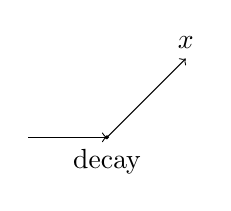
\begin{tikzpicture}
\draw[->] (0,0)--(1,0) node[draw,fill,circle,minimum size=1pt,inner sep=0,label=below:decay] {};
\draw[->] (1,0)--(2,1) node[above] {$x$};
\end{tikzpicture}
\end{frame}

\subsection{Statistiche sufficienti: teorema di fattorizzazione}\linkdest{statsuff}

\begin{frame}{Statistiche sufficienti per il parametro dato}
Statistica sufficiente $S$ per parametro $\Theta$: \keyword{sufficient statistic is a function $T(\vec{X})$ whose values contains all information needed to compute any estimate of the param}. Pdf di X data $T(X)$ non dipende da parametro $\theta$:
\[\prob{(x;S,\theta)}=\prob{(x;S)}\]
\begin{block}{Teorema di fattorizzazione}
Probabilit\'a di osservare $X$ dato $\theta$ \'e probabilit\'a di $S(x)$ dato $\theta$ per funzione sole osservabili: \[\prob{(x;\theta)}=\prob{(S(x);\theta)}h(x)\] e $\omega_{\theta}$ non dipende da $\theta$. $\vec{x}=\{x_1,\ldots,x_n\}$: $T(\vec{x})$ sufficiente iff $L(\vec{x},\theta)=g(T,\theta)h(\vec{x})$ e dominio $\omega_{\theta}$ non dipende da $\theta$. Statistiche: media campionaria $\overline{x}=\frac{\sum x_i}{N}$, varianza campionaria, etc
\end{block}
\begin{block}{Statistica sufficiente minimale}
$S$ sufficiente e esiste una funzione $f$ per ogni $s_i$ con $S=f(s_i)$ e $\dim({S})\leq\dim{(X)}$.
\end{block}
\end{frame}

\begin{frame}{Proof Neyman Factorization Theorem}
\begin{itemize}
\item $T(x_1,\ldots,x_n)$ suf. per $\theta$ ($P_{\theta}(X=x|T(X)=t(x))$ non dipende da $\theta$):
\begin{align*}
&(A): X=x,\ (B): T(X)=t(x): A\subset B\\
&L(\theta)=P_{\theta}(X=x)=P_{\theta}(X=x\cap T(X)=t(x))=P_{\theta}(T(X)=T(x))P_{\theta}(X=x|T(X)=T(x))
\end{align*}
\item $L(\theta)=g(T(x_1,\ldots,x_n);\theta)h(x_1,\ldots,x_n)$.
\begin{align*}
&p(t;\theta)=P_{\theta}(T(X)=t)=\sum_{\vec{y}:T(\vec{y})=t}\prod_if(y_i;\theta)=\sum_{\vec{y}:T(\vec{y})=t}L(\theta)\\
&P_{\theta}(X=x|T(X)=t)=g(t;\theta)h(x)/(g(t;\theta)\sum_{\vec{y}:T(\vec{y})=t}h(\vec{y}))
\end{align*}
\end{itemize}
\end{frame}

\subsection{Esempi di statistiche sufficienti}

%\begin{align*}
%&L(x;\mu,\sigma)=\frac{1}{\sqrt{2\pi}\sigma}\exp{-\frac{1}{2}\frac{(x-\mu)^2}{\sigma^2}}\\
%&\overline{x}=\frac{\sum x_i}{N}:\ %L(\overline{x};\mu)=\prod_iL(x_i;\mu,\sigma)=(\frac{1}{\sqrt{2\pi}\sigma})^N\exp{-\frac{1}{2}\frac{\sum_i(x_i-\mu)^2}{\sigma^2}}
%\end{align*}
\begin{wordonframe}{n RV iid con pdf bernoulli p}
$X_1,\ldots,X_n$: iid con pdf di Bernoulli, supporto pdf $\chi=\{0,1\}$, parametro p nell'intervallo $(0,1)$:
\begin{align*}
&T=\sum X_i\to\{0,\ldots,n\}&\intu{con pdf binomiale}
&\prob{(X_1=x_1\cap\ldots X_n=x_n|T=t)}=0, t\neq\sum x_i\\
&=\prob{(\cap_iX_i=x_i|T=t)}=\frac{\prob{((\cap_iX_i=x_i)\cap(T=t))}}{\prob{(T=t)}}=\frac{\prob{(\cap_iX_i=x_i)}}{\prob{(T=t)}}\intu{se $\sum x_i=t$:}
&A=\{\cap_iX_i=x_i\}\subseteq B=\{T=t\}
\end{align*}
e poich\'e le $X_i$ sono indipendenti si ha
\begin{align*}
&\frac{\prod\prob{(X_i=x_i)}}{\prob{(T=t)}}=\frac{p^{\sum x_i}(1-p)^{n-\sum x_i}}{\binom{n}{t}p^t(1-p)^{n-t}}
\end{align*}
\end{wordonframe}

\begin{wordonframe}{n RV iid Poisson$(\lambda)$}
$X_1,\ldots,X_n$: iid con pdf di Poisson con parametro ignoto $\lambda$:
\begin{align*}
&\prob{(X_1=x_1\cap\ldots X_n=x_n|T=t)}=\prob{(\cap_iX_i=x_i|T=t)}\\
&\frac{\prob{((\cap_iX_i=x_i)\cap(T=t))}}{\prob{(T=t)}}=\frac{\prob{(\cap_iX_i=x_i)}}{\prob{(T=t)}},\ t=\sum x_i\\
&=\frac{\prod_i[\frac{\exp{-\lambda}\lambda^{x_i}}{x_i!}]}{\frac{\exp{-n\lambda}(n\lambda)^t}{t!}}=\frac{t!}{\prod x_i!}n^{-t}
\end{align*}
\begin{block}{\keyword{Media aritmetica \'e statistica sufficiente per parametro binomiale, poissoniana, esponenziale}}
	\begin{align*}
	&\prob{(k)}=\binom{n}{k}p^k(1-p)^{n-k}\\
	&\prob{(k)}=\frac{\mu^k\exp{-\mu}}{k!}\\
	&\prob{(x)}=\lambda\exp{-\lambda x}
	\end{align*}
\end{block}
\end{wordonframe}

\begin{frame}{Statistiche suff. Gaussiana}
\begin{block}{Gaussiana: media ignota, varianza nota}
	\begin{align*}
	&L(\overline{x};\mu)=\prod_iL(x_i;\mu,\sigma)=(\frac{1}{\sqrt{2\pi}\sigma})^N\underbrace{\exp{-\frac{N}{2}\frac{\sum_i(\overline{x}-\mu)^2}{\sigma^2}}}_{g(T,\theta)}\underbrace{\exp{-\frac{N}{2}\frac{\sum_i(x_i-\overline{x})^2}{\sigma^2}}}_{h(\vec{x})}
	\end{align*}
	La statistica ''media aritmetica'' \'e sufficiente per parametro $\mu$ della gaussiana (dominio gaussiana non dipende da $\mu$) (\keyword{Ex: pdf della media aritmetica})
\end{block}
\begin{block}{Gaussiana: media nota, varianza ignota}
	$\hat{\sigma}^2=\frac{\sum x_i^2-\mu}{N}$ \'e sufficiente per $\sigma^2$ (pdf di $\hat{\sigma}^2\propto g$ e dominio gaussiana non dipende da $\sigma$). (\keyword{Ex: statistica sufficiente $\sigma$ gaussiana})
\end{block}
\end{frame}

\begin{wordonframe}{Distribuzione uniforme: \keyword{$x_{max}$ statistica sufficiente}.}
\begin{columns}[T]
\begin{column}{0.5\textwidth}
\pgfmathsetmacro{\unifM}{3}
\begin{tikzpicture}[scale=0.5,domain=0:1.5*\unifM]
\pgfmathsetmacro{\unifN}{(\unifM)^-1}
\begin{axis}[ylabel={$p(x;m)$},extra x ticks={\unifM}, extra x tick labels={$m$},
extra x tick style={xticklabel style={yshift=-10}}]
%\draw[->] (-0.2,0) -- (1.5*\unifM,0) node[right] {$x$};
%\draw[->] (0,-0.2) -- (0,1.5*\unifM) node[above,red] {$p(x;m)$};
%\draw[color=red] plot[domain=0:\unifM, id=unif] function{\unifN} node[right] {$\frac{1}{m}$};
\addplot[color=red] function [raw gnuplot, id=unifpdf, mark=none]{set xrange [0:\unifM]; plot \unifN};
\end{axis}
\end{tikzpicture}
\end{column}
\begin{column}{0.5\textwidth}
\begin{align*}
&\prob{(x;m)}=\left\{\begin{matrix}\frac{1}{m}\ x\in[0,m]\\0\\\end{matrix}\right.&\intertext{estraggo N $x_1,\ldots,x_n$}\\
&L(\vec{x},m)=\prod_iL(x_i;m)=\left\{\begin{matrix}\frac{1}{m^N}\ m>x_{max}\\0\ m<x_{max}\\\end{matrix}\right.
\end{align*}
\end{column}
\end{columns}
%$g(T,\theta)\propto A(T;\theta)$ dove $A$ \'e pdf di statistica $T$?
\begin{align*}
&\prob{(x_{max}<x_0)}=F_M(x_0)=\prod_i\prob{(x_i<x_0)}=\prod_i\int_0^{x_0}\frac{1}{m}\,dx=(\frac{x_0}{m})^N\\
&\prob{(x_M;m)}=\TDof{x_0}\left.F_M(x_0)\right|_{x_M}=\frac{N}{m}(\frac{x_M}{m})^{N-1}I(x_M<m)\\
&L_{\vec{x}}(m)=\frac{N}{m^N}x_M^{N-1}\frac{1}{Nx_M^{N-1}}=\prob{(x_M;m)}\frac{1}{Nx_M^{N-1}}\ m>x_M
\end{align*}
$\prob{(x;S,\theta)}=\prob{(x;S)}$!
\end{wordonframe}

\begin{wordonframe}{Minimo campionario per distribuzione uniforme}
\todo{Ex: distribuzione uniforme e statistica ''minimo campionario''}: Per pdf uniforme $x_{min}$ \'e sufficiente per m?
\end{wordonframe}

\begin{wordonframe}{\keyword{Statistica $x_{min}$ per pdf uniforme}}
pdf di $x_{min}$
\begin{columns}[T]
\begin{column}{0.5\textwidth}
Trasformazione di variabile
\begin{align*}
&x'\to m-x\\
&f(x_m;m)=\frac{N}{m}[1-\frac{x_m}{m}]^{N-1}I(x\leq m)
\end{align*}
\end{column}
\begin{column}{0.5\textwidth}
\keyword{Ex: pdf $x_{min}$ (cumulanti)}
\begin{align*}
&F(x_0)=\prob{[x_m>x_0]}\\
&\prob{(\{x_i\}>x_0)}=[\int_{x_0}^m\frac{dx}{m}]^N\\
&=[1-\frac{x_0}{m}]^N
\end{align*}
\end{column}
\end{columns}
\end{wordonframe}

\subsection{Statistiche sufficienti: T di Darmois}\linkdest{darmoissuff}

\begin{frame}{Teorema di Darmois}\frameintoc
\begin{block}{Teorema di Darmois: condizione necessaria e sufficiente per esistenza statistica sufficiente}
Esiste S tale che $\dim{(S)}<\dim{(X)}$ iff: pdf appartiene alla \keyword{famiglia esponenziale} e supporto non dipende dal parametro.
\begin{equation*}
p(x|\theta)=\Exp{[\sum_i^n\alpha_i(x)a_i(\theta)+\beta(x)+\gamma(\theta)}
\end{equation*}
\begin{equation*}
S_j=\sum_i\alpha_j(x_i)
\end{equation*}
$\vec{S}$ is jointly sufficient for $\theta$
\end{block}
\end{frame}


\begin{frame}{Esempi pdf esponenziale: Poisson}\frameintoc
\begin{align*}
&\frac{\exp{-\mu}\mu^k}{k!}=\exp{\mu}\exp{k\ln{\mu}}\exp{-\ln{k!}}\\
&S=\sum_i^Nk_i
\end{align*}
\end{frame}

\begin{frame}{Esempi pdf esponenziale: gaussiana media ignota}\frameintoc
\begin{align*}
&L(\overline{x};\mu)=\prod_iL(x_i;\mu,\sigma)=(\frac{1}{\sqrt{2\pi}\sigma})^N\underbrace{\exp{-\frac{N}{2}\frac{\sum_i(\overline{x}-\mu)^2}{\sigma^2}}}_{g(T,\theta)}\underbrace{\exp{-\frac{N}{2}\frac{\sum_i(x_i-\overline{x})^2}{\sigma^2}}}_{h(\vec{x})}\\
&\alpha(x)=x\ \Rightarrow\ T=\frac{1}{N}\sum x_i=\exv{X}\\
&a(\mu)=\frac{\mu}{\sigma^2}\\
&\beta(x)=-\frac{x^2}{2\sigma}\\
&c(\mu)=
\end{align*}
La statistica ''media aritmetica'' \'e sufficiente per parametro $\mu$ della gaussiana (dominio gaussiana non dipende da $\mu$) (\keyword{Ex: pdf della media aritmetica})
\end{frame}

\begin{frame}{Esempi pdf esponenziale: Gaussiana varianza ignota}
$\hat{\sigma}^2=\frac{\sum_i^N(x_i-\mu)^2}{N}$ \'e sufficiente per $\sigma^2$ (pdf di $\hat{\sigma}^2\propto g$ e dominio gaussiana non dipende da $\sigma$). (\keyword{Ex: statistica sufficiente $\sigma$ gaussiana})
\begin{align*}
&L(\overline{x};\mu)=\prod_iL(x_i;\mu,\sigma)=(\frac{1}{\sqrt{2\pi}\sigma})^N\underbrace{\exp{-\frac{N}{2}\frac{\sum_i(\overline{x}-\mu)^2}{\sigma^2}}}_{g(T,\theta)}\underbrace{\exp{-\frac{N}{2}\frac{\sum_i(x_i-\overline{x})^2}{\sigma^2}}}_{h(\vec{x})}\\
&\alpha(x)=x\mu-\frac{x^2}{2}:\ T=\sum(x_i\mu-\frac{x_i^2}{2})\\
&a(\sigma^2)=\frac{1}{\sigma^2}\\
&\beta(x)=0\ c(\sigma^2)=-\frac{\mu^2}{2\sigma^2}-\ln{(\ldots)}\\
&\hat{\sigma}^2=\frac{\sum(x_i-\mu)^2}{N}=\frac{N\mu^2-2T}{N}
\end{align*}
\end{frame}

\begin{frame}{Esempi pdf esponenziale: spazio dei parametri della Gaussiana}
\begin{align*}
&\log{\prob{(\vec{x};\mu,\sigma^2)}}=-\log{(\sqrt{2\pi}\sigma)}-\frac{x^2}{2\sigma^2}+\frac{x\mu}{2\sigma^2}+\frac{\mu^2}{2\sigma^2}\\
&\alpha_1(x)=x,\ a_1(\mu)=\mu,\ c=-\frac{\mu}{2\sigma^2}-\ln{(\sqrt{2\pi}\sigma)}\\
&\alpha_2(x)=-\frac{x^2}{2},\ a_2(\sigma^2)=\frac{1}{\sigma^2}\\
&S_{\mu}=\sum x_i,\ S_{\sigma^2}=-\sum\frac{x_i^2}{2}
\end{align*}
\keyword{Quale relazione tra numero statistiche sufficienti e parametri?}
\end{frame}

\begin{frame}{Media aritmetica \'e statistica sufficiente per parametro binomiale, poissoniana, esponenziale.}\frameintoc
\begin{columns}[T]
\begin{column}{0.33\textwidth}
\begin{align*}
&\prob{(k)}=\binom{n}{k}p^k(1-p)^{n-k}\intd{argomento di exp}
&\log{\binom{n}{k}}+k\log{\frac{p}{1-p}}\\
&+n\log{(1-p)}\\
&(\alpha(k)a(p)+\beta(k)+c(p))\\
&S=\sum_ik_i
\end{align*}
\end{column}
\begin{column}{0.33\textwidth}
\begin{align*}
&\prob{(k)}=\frac{\mu^k\exp{-\mu}}{k!}\intd{argomento di exp}
&k\log{\mu}-\mu-\log{k!}\\
&(\alpha(k)a(\mu)+\beta(k)+c(\mu))\\
&S=\sum_ik_i
\end{align*}
\end{column}
\begin{column}{0.33\textwidth}
\begin{align*}
&\prob{(x)}=\lambda\exp{-\lambda x}\intd{argomento di exp}
&-\lambda x-\mu+\log{\lambda}\\
&(\alpha(x)a(\lambda)+\beta(x)\\
&+c(\lambda))\\
&S=\sum_ix_i
\end{align*}
\end{column}
\end{columns}
\keyword{Ex: pdf non della famiglia esponenziale}: Come procedo se pdf non esponenziale (LHC)?
\end{frame}

\subsection{Stimatori puntuali}

\begin{frame}{Propriet\'a generali stiamatori}
	\begin{itemize}
		\item Consistenza (LGN): $\hat{\theta}\xrightarrow{P}\theta_0$
		\item Mean Square Error:
		\[\E{[(T-\tau(\theta))^2]}=\var{[T]}+[\E{[T]}-\tau(\theta)]^2\]
		\item Bias: $B(T)=\E{[T]}-\tau(\theta)$; scuola soggettivista: bias non esiste.
		\item Varianza $\var{\vec{X}}\propto\frac{1}{N}$, bias $b(\vec{x})$ non diminuisce all'aumentare delle misure.
		\item distribuzione semplice
	\end{itemize}
\end{frame}

\begin{frame}{Riduzione del bias}
	\begin{columns}[T]
		\begin{column}{0.5\textwidth}
			$\PDy{\theta}{b}=0$ banale: $\E{[S]}=\alpha\theta$ si pone $S'=\frac{S}{\alpha}$
		\end{column}
		\begin{column}{0.5\textwidth}
			Esempio:
			\begin{align*}
			&\E{[x_{max}]}=\frac{N}{N+1}m\\
			&b(x_M)=-\frac{1}{N+1}m\\
			&\hat{m}=\frac{N+1}{N}x_M\\
			&\var{[\hat{m}]}=(\frac{N+1}{N})^2\var{[x_M]}
			\end{align*}
		\end{column}
	\end{columns}
	\begin{columns}[T]
		\begin{column}{0.5\textwidth}
			\begin{align*}
			&\E{[S(x)]}=\theta+b(\theta)\\
			&\to\ S'(x)=S(x)-b(\hat{\theta})-\hat{b}(x)\\
			&\E{[\hat{b}(x)]}=b(\hat{\theta})\\
			&\var{[S']}=\var{[S]}+\var{[b]}
			\end{align*}
		\end{column}
		\begin{column}{0.5\textwidth}
			Metodo empirico
			\begin{align*}
			&S_N'(x)=2S_N(x)\\
			&-\frac{1}{2}[S_{\frac{N}{2}}(x_1,\ldots,x_{\frac{N}{2}})+S_{\frac{N}{2}}(x_{\frac{N}{2}},\ldots,x_N)]
			\end{align*}
			Supponendo $b_N\propto\frac{1}{N}$
			\begin{align*}
			&\E{[S_N']}=2\E{[S_N]}-\frac{1}{2}[2\E{[S_N]}]\\
			&=2\theta+\frac{2c}{N}-\frac{1}{2}[2(\theta-\frac{2c}{N})]=\theta_0+o(\frac{1}{N^2})
			\end{align*}
		\end{column}
	\end{columns}
	
\end{frame}

\begin{frame}{Stimatori puntuali: Caratteristiche stimatori}
	\begin{columns}[T]
		\begin{column}{0.4\textwidth}
			Statistica $\hat{\Theta}(X_1,\ldots,X_n)$ che fornisce stima di funzione dei parametri $\tau(\Theta)$.
		\end{column}
		\begin{column}{0.6\textwidth}
			\begin{itemize}
				\item \keyword{unbiased estimator}: $\E_{\Theta}[T]=\tau(\Theta)$
				\item \keyword{estimator bias}: $B_{\Theta}(T)=\E_{\Theta}[T]-\tau(\Theta)$
				\item \keyword{Estimator mean square error}: $\E{[(T-\tau(\Theta))^2]}=V_{\Theta}[T]+(\E{[T]}-\tau(\Theta))^2$
				\item \keyword{Stimatori consistenti}: $\lim_{n\to\infty}T_n(X_1,\ldots,X_n)\overset{P}{=}\tau(\Theta)$
			\end{itemize}
		\end{column}
	\end{columns}
\end{frame}

\begin{wordonframe}{Esempi di stimatori}
	\begin{block}{Notazione}
		$\exv{X}=\frac{S_N}{N}$. Lo stimatore \'e un RV, la stima \'e un numero determinato sulla base della misura concreta.
	\end{block}
	\begin{block}{Stimatore per $\sigma^2$ di n iid gaussiane}
		$X_1,\ldots,X_n$ n RV iid con pdf $N(\mu,\sigma^2)$. La varianza campionaria definita come $S^2=\frac{1}{n-1}\sum_i^n(x_i-\exv{X})^2$ \'e stimatore unbiased di $T(\Theta)=\sigma^2$
	\end{block}
	\begin{block}{Stimatore per $\mu$ di n iid gaussiane: CRLB per $\sigma$ noto}
		$X_1,\ldots,X_n$ n RV iid con pdf $N(\mu,\sigma^2)$. $\exv{X}\to T(\mu)=\mu$; dato che $I_{X_1}=\sigma\expy{-2}$ la media campionaria \'e CRLB $\frac{\sigma^2}{n}=V_{\mu}[\exv{X}]$.
	\end{block}
	\begin{block}{Stimatore per $\lambda$ di n iid poissoniane}
		$X_1,\ldots,X_n$ n RV iid con pdf $P(\lambda)$. $\exv{X}$ \'e stimatore di $T(\lambda)=\lambda$, $V_{\lambda}[\exv{X}]=\frac{\lambda}{n}$ quindi si raggiunge CRLB $\frac{\lambda}{n}$ ($I_{X_1}(\lambda)=\invers{\lambda}$).
	\end{block}
	\begin{block}{Stimatore per $p$ di n iid Bernoulli}
		$X_1,\ldots,X_n$ n RV iiir has received mainly positive reviews. d con pdf $B(p)$. $\exv{X}$ \'e unbiased estimator of $\tau(p)=p$; dato che $I_{X_1}(p)=\frac{1}{p(1-p)}$, con $X_p[\exv{X}]=\frac{p(1-p)}{n}$ siamo al CRLB $\frac{p(1-p)}{n}$.
	\end{block}
	\begin{block}{Stimatori upper limit pdf uniforme: media aritmetica vs $x_{max}$.}
		\begin{columns}[T]
			\begin{column}{0.4\textwidth}
				\begin{align*}
				&\hat{m}_1=\frac{S_N}{N}=2\exv{X}\\
				&b=\E{[\hat{m}_1]}-m=0\\
				&\var{[\hat{m}_1]}=\frac{4Nm^2}{12N^2}
				\end{align*}
			\end{column}
			\begin{column}{0.6\textwidth}
				\begin{align*}
				&p(x_{max};m)=\frac{N}{m^N}x_m^{N-1}\\
				&\E{[x_{max}]}=\int_0^m\frac{N}{m^N}x_m^N\,dx_m=\frac{N}{N+1}\frac{m^{N+1}}{m^N}\intu{asintoticamente unbiased}
				&\E{[x_{max}^2]}=\frac{N}{N+2}m^2-\frac{N^2}{(N+1)^2}m^2\\
				&\var{[x_m]}=\E{[x_m^2]}-\E^2{[x_m]}\to0\\
				&b(x_m)=-\frac{1}{N+1}m
				\end{align*}
			\end{column}
		\end{columns}
	\end{block}
\end{wordonframe}

\section{Informazione, statistiche sufficienti e MVB}

\subsection{Informazione}\linkdest{informazione}

\begin{frame}{Informazione di Fischer}
Informazione contenuta nei dati su un parametro $\Theta$
\begin{align*}
&\overbrace{I_X(\Theta)}^{\text{n RV iid:}=nI_{X_1}}=\E_{\Theta}{[(\PDof{\Theta}\log{f(X;\Theta}))^2]}=\overbrace{-\E_{\Theta}{[\PtwoDof{\Theta}\log{f(X;\Theta)}]}}^{\text{se esistono finiti $\PtwoDof{\Theta}$ e $\E{}$}}
\end{align*}
Per due parametri:
\begin{align*}
&I_X(\Theta)=\begin{pmatrix}I_{11}(\Theta)&I_{12}(\Theta)\\I_{21}(\Theta)&I_{22}(\Theta)\end{pmatrix}\ I_{ij}(\Theta)=-\E{[\frac{\partial^2}{\partial\Theta_i\partial\Theta_j}\log{f(X;\Theta)}]}
\end{align*}
\begin{block}{Score statistics}
	\begin{columns}[T]\begin{column}{0.5\textwidth}
			
		\end{column}\begin{column}{0.5\textwidth}
			
	\end{column}\end{columns}
\end{block}
\end{frame}

\begin{frame}{Qualcosa su Informazione}
\begin{block}{Informazione e statistiche}
$I_X(\Theta)\geq I_T(\Theta)$: l'uguaglianza vale iff T \'e sufficiente per $\Theta$.
\end{block}
\begin{align*}
&Y=h(X)\ 1-1 \Rightarrow I_X=I_Y\\
&X\to f(X;\Theta)\ Y\to g(Y;\Theta)=f(\invers{h}(Y);\Theta)|\TDy{y}{\invers{h}(Y)}|\\
&I_Y=\E_Y{[(\PDof{\Theta}\log{g(Y)})^2]}=\E_Y{[(\PDof{\Theta}\log{f(\invers{h}(Y)})^2]}\\
&=\E_X{[(\PDof{\Theta}\log{f(X)})^2]}
\end{align*}
\end{frame}

\begin{wordonframe}{Esempi Informazione}
\begin{columns}[T]
\begin{column}{0.5\textwidth}
	\begin{block}{pdf Poisson}
		\begin{align*}
		&\log{f}=-\lambda+x\log{\lambda}-\log{x!}\\
		&I_X(\lambda)=\invers{\lambda}
		\end{align*}
	\end{block}
\end{column}
\begin{column}{0.5\textwidth}
	\begin{block}{pdf Gauss}
		\begin{align*}
		&\log{f}=-\frac{1}{2}\frac{(x-\mu)^2}{\sigma^2}-\log{(\sqrt{2\pi}\sigma)}\\
		&I_X(\mu)=\sigma\expy{-2}
		\end{align*}
	\end{block}
\end{column}
\end{columns}
\begin{block}{n RV iid}
\begin{columns}[T]
	\begin{column}{0.5\textwidth}
		$X_1,\ldots,X_n$ n RV iid:
		\begin{align*}
		&X=\sum X_i\\
		&I_X(\Theta)=nI_{X_1}(\Theta)
		\end{align*}
	\end{column}
	\begin{column}{0.5\textwidth}
		proof pg 327 probability and statistical inference
	\end{column}
\end{columns}
\end{block}
\begin{block}{n RV gaussiane $N(\mu,\sigma^2)$: matrice informazione}
$\vec{X}=(X_1,\ldots,X_n)$ e $\vec{\Theta}=(\mu,\sigma^2)$
\begin{align*}
&I_{11}=\E{[(\PDof{\mu}\log{f})^2]}=\sigma\expy{-2}\ I_{22}=\E{[(\PDof{\sigma^2}\log{f})^2]}=\frac{1}{2}\sigma\expy{-4}\\
&I_{12}=I_{21}=\frac{1}{2\sigma^2}\E{[\sigma\expy{-3}(X_1-\mu)^3-(X_1-\mu)]}=0
\end{align*}
\end{block}
\begin{block}{Perdita di informazione se tengo solo media campionaria delle RV gaussiane}
$\vec{X}=(X_1,\ldots,X_n)$ e media $\exv{X}=\frac{1}{n}\sum X_i$ con pdf $N(\mu,\invers{n}\sigma^2)=g(x,\Theta)=\frac{\sqrt{n}}{\sigma\sqrt{2\pi}}\exp{-\frac{n}{2\sigma^2}(x-\mu)^2}$
\begin{align*}
&I_{11}=\E{[(\PDof{\mu}\log{g})^2]}=n\sigma\expy{-2}\ I_{22}=\E{[(\PDof{\sigma^2}\log{g})^2]}=\frac{1}{2}\sigma\expy{-4}\\
&I_{12}=I_{21}=\frac{1}{2\sigma^2}\E{[\sigma\expy{-3}(X_1-\mu)^3-(X_1-\mu)]}=0\\
&I_{\vec{X}}-I_{\exv{X}}\geq0
\end{align*}
\end{block}
\begin{block}{Perdita di informazione se tengo solo la varianza campionaria delle RV gaussiane}
Varianza campionaria $S^2=\frac{1}{n-1}\sum_i(X_i-\exv{X})^2$ (\keyword{Gaussian variance: unbiased estimator}). 
La RV $Y=(n-1)\frac{S^2}{\sigma^2}$ ha pdf $\chi^2_{n-1}$: $c\exp{-\frac{1}{2}y}y\expy{\frac{n-3}{2}}$ con $c=2\expy{\frac{n-1}{2}}\Gamma(\frac{1}{2}(n-1))$
\begin{align*}
&S^2\to h(x;\theta)=d\sigma\expy{-(n-1)}\exp{-\frac{n-1}{2}\frac{x}{\sigma^2}}x\expy{\frac{n-3}{2}}\ d=c(n-1)^{\frac{n-1}{2}}\\
&I_{11}=I_{12}=I_{21}=0\ I_{22}=\frac{1}{2}(n-1)\sigma\expy{-4}:\\ &I_{\vec{x}}-I_{S^2}=\begin{pmatrix}n\sigma\expy{-2}&0\\0&\frac{1}{2}\sigma\expy{-4}\end{pmatrix}''\geq0''
\end{align*}
$\exv{X}$, $S^2$ are indipendently ($P(A\cap B)=P(A)P(B))$) distributed: $I_{\exv{X},S^2}=I_{\exv{X}}+I_{S^2}=I_{\vec{X}}(\Theta)$.
\end{block}
\begin{block}{Poissoniana}
$k_1,\ldots,k_n$ n RV iid poissoniane $f(k,\mu)=\frac{\mu^k\exp{-\mu}}{k!}$:
\begin{align*}
&I_k(\mu)=-\E{[\PtwoDy{\mu}{\log{(L)}}]}=N(-\E{[\PtwoDy{\mu}{\log{(p(k;\mu))}}]})\\
&\PtwoDy{\mu}{\log{(p(k;\mu)}}=-\frac{k}{\mu^2}\\
&I_k(\mu)=N\E{[\frac{k}{\mu}]}=\frac{N}{\mu}\\
&S=\sum k_i,\ f(S;\mu)=\frac{(N\mu)^S\exp{-N\mu}}{S!},\ I_s(\mu)=\frac{N}{\mu}
\end{align*}
$I_s=I_k$ poich\'e $S$ \'e statistica sufficiente.
\end{block}
\begin{block}{Binomiale}
\begin{align*}
&I_k(p)=-N\E{[\PtwoDy{p}{\log{f(k;n,p)}}]}=N\frac{n}{p(1-p)}\\
&S=\sum_ik_i:\ f(S;nN,p)=\binom{nN}{S}p^S(1-p)^{nN-S}
\end{align*}
\keyword{Ex: Informazione di binomiale e statistica suff.}
\end{block}
\begin{block}{Ex: Pdf uniforme e minimum variance bound per $x_M$}
\begin{align*}
&I_{X_1}=I_{x_m}(m)=\frac{N^2}{m}\\
&\var{[\hat{\theta},\theta]}=\frac{N}{(N+2)(N+1)^2}m\overset{??}{\geq}\frac{(1+\TDy{\theta}{b})^2}{I_{\hat{\theta}}(\theta)}=\frac{(1-\frac{1}{N+1})^2}{\frac{N^2}{m^2}}
\end{align*}
\keyword{Ex: Pdf uniforme e minimum variance bound per $x_m$}
\end{block}
\framebreak
\begin{block}{Statistica $x_m$ non \'e consistente}
\begin{align*}
&\E{[x_m]}=\int\,dx_mx_mf(x_m;m)=\int\,dx_mx_m\frac{N}{m}[1-\frac{x_m}{m}]^{N-1}=\frac{m}{N+1}\\
&\E{[x_m^2]}=\int\,dx_mx_m^2f(x_m;m)=\int\,dx_mx_m^2\frac{N}{m}[1-\frac{x_m}{m}]^{N-1}\\
&=\frac{2m^2}{(N+1)(N+2)}\\
&\var{[x_m]}=\E{[x_m^2]}-\E^2{[x_m]}=\frac{N}{(N+1)^2(N+2)}m^2\to0\\
&\hat{m}=(N+1)x_m:\ \E{[\hat{m}]}=m,\ \var{[\hat{m}]}=\frac{N^2}{(N+1)(N+2)}m^2\\
&I_{x_m}(m)=\frac{N}{(N-2)m^2},\ (CR:\ \frac{N}{N+2}\geq\frac{N-2}{N})
\end{align*}
$\hat{m}$ non \'e consistente: non converge in probabilit\'a al parametro.
\end{block}
\end{wordonframe}

\begin{frame}{Come ridurre i dati se statistica sufficiente non \'e disponibili}
Perdita informazione
\begin{itemize}
\item istogramma
\item dati troncati, $r=\frac{1}{2}-\frac{n_r}{N}$.
\item media windsorizzata
\end{itemize}
\end{frame}

\subsection{Unbiased best estimator}

\begin{wordonframe}{Teorema di Rao-Blackwell}
	T is unbiased estimator of $\tau(\theta)$, U if jointly sufficient statistics for $\theta$ and $g(u)=\E{[T|U=u]}$: $W=g(U)$ is unbiased estimator of $\tau(\theta)$ $\var{[W]}\leq\var{[T]}$.
	Proof:
	\begin{align*}
	&\E{[X]}=\E_Y{[\E{[(X|Y)]}]}\\
	&\tau(\theta)=\E_{\theta}{[T]}=\E_U{[\E{[T|U]}]}=\E{[g(u)]}=\E_{\theta}{[W]}\\
	&\var{[T]}=\E{[(T-\tau(\theta))^2]}=\E{[(W-\tau(\theta))^2]}+\E{[(T-W)^2]}\\
	&+2\E{[(T-W)(W-\tau(\theta))]}\\
	&\E{[(T-W)(W-\tau(\theta))]}=\E_U{[\E{[(T-g(U))(g(U)-\tau(\theta))|U]}]}\\
	&=\E_U{[(T-g(U))\E{[(g(U)-\tau(\theta))|U]}]}=0
	\end{align*}
\end{wordonframe}

\begin{frame}{Best unbiased estimator}\frameintoc\linkdest{cramerrao}
	\begin{block}{\keyword{Disuguaglianza di Cramer-Rao (CRLB)}}
		$X_1,\ldots,X_n$ iid con pdf $f(x,\Theta)$: se supporto $\Omega_{\Theta}$ di $f(x,\Theta)$ non dipende da $\Theta$ e integrali in $dx$ sono invertibili con $\PDof{\Theta}$; esiste stimatore unbiased $T(\vec{X})\xrightarrow{\E{[\ ]}}\tau(\Theta)$ con $\PDy{\Theta}{\tau}$ esiste finito, allora:
		\begin{align*}
		&V_{\Theta}[T]\geq\frac{[\tau'(\Theta)]^2}{n\E_{\Theta}[(\PDof{\Theta}\log{f(X_1;\Theta)})^2]}=\frac{[\tau'(\Theta)]^2}{nI_{X_1}(\Theta)}\\
		&\E{[T-\tau(\theta)]}=\var{[T]}+\overbrace{[\E{[T]}-\tau(\theta)]^2}^{b^2}: \left(\frac{(1+\TDy{\theta}{b})^2}{I_{\hat{\Theta}}(\theta)}\right)
		\end{align*}
		(\keyword{minimum variance bound})
	\end{block}
	\begin{block}{Best unbiased estimator}
		Uniformly minimum variance unbiased estimator such that $V_{\Theta}[T]\leq V_{\Theta}[T*]$ for all estimator $T^*$ unbiased.
	\end{block}
\end{frame}

\begin{frame}[t]{Dimostrazione CRLB}
	\begin{align*}
	&\tau(\theta)=\int_{\chi}T(X_1,\ldots,X_n)\underbrace{\prod_if(X_i;\theta)}_{\Exp{\sum_i\log{f(X_i;\theta)}}}\,dx_i\\
	&\tau'(\theta)=\int_{\chi}T(X_1,\ldots,X_n)\underbrace{[\PDof{\theta}\prod_if(X_i;\theta)]}_{\sum_i\PDof{\theta}[\log{f(X_i;\theta)}]\prod_if(X_i;\theta)}\prod_i\,dx_i\\
	&=\E{[TY]},\ Y=\sum_i\PDof{\theta}[\log{f(X_i;\theta)}]\\
	&\E{[Y]}=\E{[\sum_i\PDof{\theta}(\log{f(X_i;\theta)})]}=0=\sum_i\PDof{\theta}\int_{\chi}f(X_i;\theta)\,dx\\
	&\tau'^2=\cov^2{(T,Y)}=(\E{[TY]}-\E{[T]}\cancelto{0}{\E{[Y]}})^2\leq \var{[T]}\var{[Y]}\\
	&\var{[Y]}=\E{[Y^2]}=n\E{[(\PDof{\theta}\log{f(X_i;\theta)})^2]}
	\end{align*}
\end{frame}

\begin{frame}{Best Linear Uniform Estimators (\keyword{BLUE})}
	$T_i$: k stimatori unbiased di $\tau(\theta)$, $\var{[T_i]}=\delta^2<\infty$, $T_i$ pairwise uncorrelated. Estimator with smallest variance in
	\[D=\{T=\sum_i^k\alpha_iT_i,\ \sum_i\alpha_i=1\}\]
	is for $\alpha_i=\invers{k}$: $\frac{1}{k}\sum_i^kT_i$
\end{frame}

\section{Metodi costruzione stimatori consistenti}\linkdest{methodsestimators}

\begin{frame}{Utilizzo LLN per costruzione stimatori consistenti}\frameintoc
Consistenza: $\hat{\theta}\xrightarrow{P}\theta_0$. Una quantit\'a con queste caratteristiche \'e
\[\invers{N}\sum_ia(X_i)\xrightarrow{N\to\infty}\E{[a(X)]}=\int a(X)f(X;\theta)\,dX=h(\theta)\]
dove $a(X)$ \'e qualsiasi funzione di X con varianza finita: per LLN sample mean is C-estimator of $a(X)$. Se per $\theta_0$ esiste la funzione inversa $\invers{h}[h(\theta_0)]=\theta_0$ si ha $\hat{\theta}=\invers{h}[\invers{N}\sum_i^Na(X_i)]$
Most used methods making use of LLN:
\begin{itemize}
\item Moments methods
\item Maximum likelihood method
\item Least square method
\end{itemize}
\end{frame}

\subsection{Metodo dei momenti}

\begin{frame}{Stimatori Consistenti: Metodo dei Momenti (Cowan 128/James 131)}\frameintoc
Semplice computazionalmente - Ho N osservazioni $x_1,\ldots,x_n$ di RV iid con pdf $f(x,\theta)$, $\theta=(\theta_1,\ldots,\theta_m)$. Cerco m funzioni linindip $a_i(X)$:
\[\E{[a_i(x)]}=\int a_i(x)f(x;\theta)\,dx=h_i(\theta)\to\frac{\sum_i\E{[x_i^k]}}{N}\]
Se $a_j(X_i)=X^j$ $h_j(\theta)$ sono i momenti della distribuzione $\mu_j'(\theta)$.
%\begin{columns}[T]
%\begin{column}{0.65\textwidth}
%\begin{align*}
%&\cov{(m_i,m_j)}=\E{[m_im_j]-\E{[m_i]}\E{[m_j]}}\\
%&=\frac{\mu'_{i+j}-\mu_i'\mu_j'}{N}\\
%&\cov{[\hat{\theta}_i,\hat{\theta}_j]}=\sum_{k,l}\PDy{\hat{e}_k}{\hat{\theta}_i}\PDy{\hat{e}_l}{\hat{\theta}_j}\cov{[\hat{e}_k,\hat{e}_l]}
%\end{align*}
%Co-var matrix of estimators (error propagation formula)
%\end{column}
%\begin{column}{0.35\textwidth}
%\begin{align*}
%&m_1=\mu_1'(\theta_1,\ldots,\theta_n)\\
%&\vdots\\
%&m_n=\mu_n'(\theta_1,\ldots,\theta_n)\intd{Invertendo il sistema sopra si trovano gli stimatori:}
%&\hat{\theta_1}(m_1,\ldots,m_m)\\
%&\vdots\\
%&\hat{\theta_m}(m_1,\ldots,m_m)
%\end{align*}
%\end{column}
%\end{columns}
\end{frame}

\subsection{stimatori impliciti}

\begin{frame}{\keyword{Stimatori impliciti}: generalizzazione del metodo dei momenti}
We find $a(X,\theta)$ in maniera che $h(\theta_0)=0$ per il valore vero di $\theta_0$
\[\E{[a(X,\theta_0)]}=\int a(X,\theta_0)f(X,\theta_0)dX=h(\theta_0)=0\]
Per LLN \[\xi(\theta_0)=\frac{1}{N}\sum_ia(X_i,\theta_0)\xrightarrow{N\to\infty}\E{a(X,\theta_0)}=0\]
One of the root of $h(\theta)$ give consistent estimate of $\theta_0$ if $\xi$ is differentiable, mean of $\xi$, $\PDy{\theta}{\xi}$ exist and $\lim_{N\to\infty}\E{[\PDy{\theta}{\xi(\theta)}]_{\theta=\theta_0}}\neq0$.
In practice one find $a(X_i,\theta)$ minimizing other function g: $a(X_i,\theta)=\PDof{\theta}g(X_i,\theta)$ (maximum likelihood and minimum $\chi^2$).
Metodo momenti: $a(X_i,\theta)\to a(X_i)-\E{[a(X)]}$.
\end{frame}

\begin{wordonframe}{Examples moment estimators}
\begin{columns}[T]\begin{column}{0.5\textwidth}
\begin{block}{Uniforme $U(a,b)$}
\begin{align*}
&\mu_1=\E{[X]}=\frac{1}{2}(a+b)\\
&\mu_2=\E{[X^2]}=\frac{1}{3}(a^2+ab+b^2)\\
&\hat{a}=\mu_1\pm\sqrt{3(\mu_2-\mu_1^2)}\\
&\hat{b}=2\mu_1-a
\end{align*}
\end{block}
\end{column}\begin{column}{0.5\textwidth}

\end{column}\end{columns}
\end{wordonframe}

\subsection{Stimatori di massima likelihood (MLE)}

\begin{frame}{Stimatori di massima likelihood: Likelihood equation}\linkdest{MLE}\frameintoc
\begin{align*}
&a(X,\theta)=\PDy{\theta}{\log{L}}=\PDof{\theta}g(X_i,\theta)\\ &\xi(\theta)=K_N=\frac{1}{N}\PDof{\theta}\sum_i^Ng(X_i,\theta)=\frac{1}{N}\sum_i\PDy{\theta}{\log{(L(x_i,\theta))}}=0\\
&\PDof{\theta}\sum_i^N\ln{f(X_i,\theta)}=\PDof{\theta}\ln{L(\vec{X},\theta)}=0 \tag*{(Likelihood equation)}
\end{align*}
Condizione necessaria per massimo di $L(\vec{X},\theta)$ se non si ha sul bordo di $\Theta$: una radice \'e stimatore consistente se $f$ \'e  2-differenziabile risp $\theta$, le medie delle due prime derivate esistono e l'integrazione risp $\vec{X}$ e la derivata risp $\theta$ commutano. The quantity $\PDof{\theta}\ln{L(\vec{X},\theta)}\to G(0,NI_{X_1}(\theta))$: massimo assoluto (asintotico) \'e consistente.
\end{frame}

\begin{wordonframe}{Radice equazione di likelihood \'e stimatore consistente}
\begin{align*}
&\E{[\PDof{\theta}\ln{f(X,\theta)}]}|_{\theta=\theta_0}=0\tag{normalizzazione}\\
&\int\PtwoDy{\theta}{\ln{f}}f\,dX+\int(\PDy{\theta}{\ln{f}})^2f\,dX=0\tag{differenziando ancora}
\end{align*}
Differenziando la grandezza sperimentale $K_N=\frac{1}{N}\PDof{\theta}\sum_i^Ng(X_i,\theta)=\xi(X_i,\theta)$
\begin{align*}
&\E{[\PDy{\theta}{\xi}|_{\theta_0}]}=\E{[\frac{1}{N}\PtwoDy{\theta}{\ln{L(\vec{X},\theta)}}|_{\theta_0}]}\\
&\E{[\PDy{\theta}{\xi}|_{\theta_0}]}\xrightarrow{N\to\infty}\E{[\PtwoDy{\theta}{\ln{f(X,\theta)}}|_{\theta_0}]}=-\E{[(\PDy{\theta}{\ln{f(X,\theta)}})^2]}=-I_X<0\\
%&\E{[\PDy{\theta}{K}]}=\E{[\PtwoDy{\theta}{\log{L}}]}=-\E{[(\PDy{\theta}{\ln{f(X,\theta)}})^2]}=-I_X<0
\end{align*}
\begin{align*}
&\int f(X,\theta_0)\ln{[\frac{f(X,\theta)}{f(X,\theta_0)}]}\,dX\\
&<\ln{\int f(X,\theta_0)\frac{f(X,\theta)}{f(X,\theta_0)}\,dX}=0:\ \theta\neq\theta_0\tag{ln strictly concave}\\
&\lim_{N\to\infty}\frac{1}{N}\sum_i^N\ln{f(X_i,\hat{\theta}_N')}=\E{[\ln{f(X_i,\lim_{N\to\infty}\hat{\theta}_N')}]}\tag{$\hat{\theta}_N'$ non-C sols.}\\
&<\E{[\ln{f(X,\theta_0)}]}=\lim_{N\to\infty}\frac{1}{N}\sum_i^N\ln{f(X_i,\hat{\theta}_N)}
\end{align*}

\end{wordonframe}

\begin{frame}[allowframebreaks]{Propriet\'a MLE}
\begin{block}{Consistente se soluzione della likelihood equation \'e unica: massimo assoluto (asintotico) \'e consistente}
$\PDy{\theta}{\log{L_{tot}}}=0$.
\end{block}
\begin{block}{Invariante per trasformazione di parametro}
\end{block}
\begin{block}{Asintoticamente un-biased}
\end{block}
\begin{block}{Asintoticamente efficente: $\var{[\hat{\theta}]}\to\frac{1}{NI_{X_1}}$}
\begin{align*}
&K_N(\hat{\theta)}=K(\theta_0)+\PDy{\theta}{K_N}(\hat{\theta}-\theta_0)+o(\hat{\theta}-\theta_0)^2\intd{prendendo il valore di aspettazione}
&0=\sum_i\frac{\PDy{\theta}{\log{(L(x_i))}}}{N}-I(\hat{\theta}-\theta_0)+(\var{[\hat{\theta}]})\\
&\hat{\theta}-\theta_0\propto N(0,\frac{1}{NI})+\frac{\const{}}{N}: \lim_{N\to\infty}b(\hat{\theta})\propto\frac{1}{N}
\end{align*}
\end{block}
\begin{block}{Pdf dello stimatore tende asintoticamente ad gaussiana}
\end{block}
\begin{block}{MLE per pdf esponenziale}
Per pdf esponenziale\[f(x;\theta)=\exp{\alpha(x)a(\theta)+\beta(x)+c(\theta)}\] il metodo di massima likelihood determina lo stimatore efficiente e senza bias $\hat{M}=\frac{1}{N}\sum_i\alpha(x_i)$ di $M(\theta)=-\frac{\TDy{\theta}{c(\theta)}}{\TDy{\theta}{a(\theta)}}$.
\end{block}
\cite{barlow1990extended}
\end{frame}

\begin{frame}{Likelihood for binned data}
%N fissato
%\begin{align*}
%&\prob{(\vec{k},\theta)}=\frac{N!}{\prod_ik_i!}\prod_i{\underbrace{\prob{(i)}}_{\int_{S_i}\prob{(x|\theta)}\,dx}}\mkern-20mu^{k_i}\\
%&\max{[\sum_i k_i\log{[\prob{(x;\theta)}\Delta]}]}\\
%&\to\max{[\sum_i \log{[\prob{(n_i;\theta)}]}]}
%\end{align*}
\begin{block}{Multinomial model of data}
\begin{align*}
&\vec{n}=(n_1,\ldots,n_N),\ n_T=\sum^Nn_i\\
&\vec{\nu}=(\nu_1,\ldots,\nu_N),\ \nu_T=\sum^N\nu_i\\
&\nu_i(\theta)=\nu_T\int_{bin i}f(x;\theta)\,dx\\
&f(\vec{n},\theta)=\frac{n_T!}{n_1!\ldots n_N!}(\frac{\nu_1}{n_T})^{n_1}\ldots(\frac{\nu_N}{n_T})^{n_N}\\
&L(\theta)=\sum^Nn_i\ln{\nu_i(\theta)}
\end{align*}
\end{block}
\begin{block}{Poissonian model of data}
Extended Likelihood
\end{block}

Fit resolution of histogram (??): $A=\sum_i\frac{1}{P_i}(\PDy{\theta}{P_i})^2$
\end{frame}

\begin{frame}{\keyword{Extended likelihood}}
La normalizzazione \'e data dal numero di eventi attesi $\mathcal{N}(\theta)$: gli eventi osservati N fluctuates as Poisson
%\begin{align*}
%&\mu_i=\mu_TP_i(\theta)\\	&\prob{(k_i;\theta)}=\frac{\prod_i\exp{-\mu_TP_i}(\mu_TP_i)^{k_i}}{k_i!}\\
%&\log{L}=\sum_ik_i\log{P_i(\theta)}+k_i\log{\mu_T}\\	&-\mu_TP_i-\bcancel{\log{k!}}\\
%&\left\{\begin{matrix}\mkern-240mu\PDy{\theta_i}{\log{L}}=0\\\PDy{\mu_T}{\log{L}}=0\ (:L(\bcancel{\mu_T}),\mu_T(\bcancel{\theta_i}) \Rightarrow\ \mu_T=N)\\\end{matrix}\right.
%\end{align*}
$\Delta x$ such that 0/1 event per bin: Poisson statistics say that $P_0(x)=\exp{-\Delta xP(x)}$, $P_1(x)=\Delta xP(x)\exp{-\Delta xP(x)}$; inlimit $\Delta x\to dx$
\begin{align*}
&L=\prod_{bin i: 1}\Delta xP(x_i)\prod_j\exp{-\Delta xP(x_j)}\to\prod_iP(x_i)d^Nx\exp{-\mathcal{N}}\\
&\ln{L}=\sum\ln{P(x_i)}-\mathcal{N}(\theta)
\end{align*}
oppure
\begin{align*}
&L=\prod_i(x_i)\exp{-\mathcal{N}}\frac{\mathcal{N}^N}{N!}\\
&L=\prod_iP(x_i)\frac{\exp{-\mathcal{N}}}{N!}\ (P(x)=\mathcal{N}p(x))
\end{align*}
\end{frame}

\begin{wordonframe}{Esempi di stimatori di massima likelihood}
\keyword{Binomiale: $K_1,\ldots,K_N:\ f(k;n,p)=\binom{n}{p}p^k(1-p)^{n-k}$}
\begin{align*}
&\log{(L(\vec{k},p))}=\log{[\prod_i^N\binom{n}{k_i}p^{k_i}(1-p)^{n-k_i}]}\\
&\max{(L)}:\ \TDof{p}\log{(L)}=\sum_i^N[\frac{k_i}{p}+(n-k_i)\frac{(-1)}{1-p}]=0\Rightarrow\sum^Nk_i=Nnp\\
&\hat{p}_{MLE}=\sum\frac{k_i}{Nn}=\exv{k}\\
&\E{[\hat{p}]}=\frac{1}{N}\frac{\sum\E{[k_i]}}{n}=\frac{\sum^Npn}{nN}=p\\
&\var{[\hat{p}]}=\var{[\frac{1}{nN}\sum k_i]}=\frac{1}{n^2N^2}Nnp(1-p)\\
&I_{k_i}(p)=\frac{nN}{p(1-p)}\to\frac{1}{\var{}}: MVB
\end{align*}

\keyword{Gaussiana}
Ho N misure $x_i$ da RV con distro gaussiana: cerco MLE per $\mu, \sigma^2$.
\begin{columns}[T]
\begin{column}{0.5\textwidth}
\begin{align*}
&G(x;\mu,\sigma)=\frac{1}{\sqrt{2\pi\sigma^2}}\exp{-\frac{(x-\mu)^2}{2\sigma^2}}\\
&\log{L}=-N\log{\sigma}-\frac{1}{2\sigma^2}\sum_i^N(x_i-\mu)^2\\
&\E{[\hat{\sigma^2}]}=\frac{1}{N}\sum_i\E{[x_i^2-2x_i\exv{x}+\exv{x}^2]}\\
&\E{[x_i^2]}=\mu^2+\sigma^2\\
&\E{[x_i\exv{x}]}=\frac{1}{N}\E{[x_i^2+\sum_{j\neq i}x_ix_j]}\\
&\E{[\exv{x}^2]}=\E{\frac{\sum x_i\sum x_j}{N^2}}=\mu^2+\frac{\sigma^2}{N}
\end{align*}
\end{column}
\begin{column}{0.5\textwidth}
Maximum of $\log{L}$ for $\mu, \sigma^2$
\begin{align*}
&\PDy{\mu}{\log{L}}=0\\
&\hat{\mu}=\frac{\sum x_i}{N}\\
&\PDy{\sigma}{\log{L}}=0\\
&-\frac{N}{\sigma^2}+\frac{1}{\sigma^4}\sum^N(x_i-\exv{x}(\to\mu))=0\\
&\hat{\sigma^2}=\frac{\sum(x_i-\exv{x})^2}{N}\intd{T darmois in 2D: stat. suff.:}
&\sum x_i,\ \sum x_i^2
\end{align*}
\end{column}
\end{columns}
$\E{[\hat{\sigma^2}]}=\frac{N-1}{N}\sigma^2$ quindi definisco lo stimatore unbiassato $\hat{\sigma^2}'=\frac{\sum(x_i-\exv{x})^2}{N-1}$.

\begin{columns}[T]
\begin{column}{0.6\textwidth}
\keyword{Esponenziale: cambio di parametro.} $p(x;\tau)=\frac{1}{\tau}\exp{-\frac{x}{\tau}}=\lambda\exp{-\lambda x}=p(x;\lambda)$:
\end{column}
\begin{column}{0.4\textwidth}
likelihood \'e invariante per cambio di parametro
\end{column}
\end{columns}
\begin{columns}[b]
\begin{column}{0.4\textwidth}
$\hat{\tau}_{MLE}=\frac{\sum_ix_i}{N}:\ \E{[\hat{\tau}]}=\tau,\ I_x(\tau)=\frac{1}{\var{\hat{\tau}}},\ \var{\hat{\tau}}=\frac{\tau^2}{N}$
\end{column}
\begin{column}{0.6\textwidth}
$\log{L}=N\log{\lambda}-\lambda\sum_ix_i$, $\TDy{\lambda}{\log{\lambda}}=0$. $\hat{\lambda}=\frac{N}{\sum x_i}=\frac{1}{\hat{\tau}}$, $\E{[\hat{\lambda}]}=\frac{N}{N-1}\lambda$
\end{column}
\end{columns}
\begin{align*}
&\phi_x(k)=\E{[\exp{ikx}]}=\intzi\exp{ikx}\exp{-\lambda x}\lambda\,dx=\frac{1}{1-i\frac{k}{\lambda}}\\
&\phi_{\sum x_i}\frac{1}{(1-\frac{ik}{\lambda})^N},\ z=\sum x_i\ \text{distribuzione di Erlang}\downarrow\\
&\prob{(z)}=\frac{1}{2\pi}\intsinf{}\frac{\exp{-ikz}}{(1-\frac{ik}{\lambda})^N}\,dk=\frac{\lambda^N}{(N-1)!}z^{N-1}\exp{-\lambda z}
\end{align*}
\begin{columns}[T]
\begin{column}{0.65\textwidth}
\begin{align*}
&\var{[\hat{\lambda}]}=\frac{N^2}{(N-1)^2(N-2)}\lambda^2\to\frac{\lambda^2}{N}\\
&M(\lambda)=-\frac{\TDy{\lambda}{c(\lambda)}}{\TDy{\lambda}{a(\lambda)}}=-\frac{\frac{1}{\lambda}}{-1}=\frac{1}{\lambda}
\end{align*}
\end{column}
\begin{column}{0.35\textwidth}
\begin{align*}
&\alpha(x)=x\\
&a(\lambda)=\lambda\\
&\beta(x)=0\\
&c(\lambda)=\log{\lambda}
\end{align*}
\end{column}
\end{columns}
\keyword{Ex: pdf di $\frac{1}{\sum x_i}$: funzione caratteristica o ''convoluzione''}
\keyword{Ex: Cambiamento di variabile pdf Erlang}
\begin{align*}
&z\to\frac{z}{N}=\exv{x}=\hat{\tau}\\
&\exv{x}\to\frac{1}{\exv{x}}=\hat{\lambda}
\end{align*}

\keyword{Ex: MLE per $x_{max}$ e $x_{min}$ per pdf uniforme}
Per $x_{min}$: \[p(x_{min},m)=\frac{N}{m}[1-\frac{x_{min}}{m}]^{N-1}\] con $x_{min}\in[0,m]$,
\begin{align*}
&\log{L}=\log{N}-\log{m}+(N-1)\log{(1-\frac{x_{min}}{m})}\\
&\TDy{m}{\log{L}}=-\frac{1}{m}+(N-1)\frac{1}{1-\frac{x_{min}}{m}}(\frac{-1}{m^2})=0\\
&\hat{m}_{MLE}=Nx_{min}:\ \E{[\hat{m}]}=\frac{N}{N+1}m,\ \var{\hat{m}}=\frac{N^3}{(N+1)^2(N+2)}m^2
\end{align*}
lo stimatore non \'e consistente.

\keyword{MLE per poissoniana}
\begin{align*}
&P(k;\mu)=\frac{\mu^k\exp{-\mu}}{k!}\\
&
\end{align*}
\end{wordonframe}

%\begin{wordonframe}{MLS refs}
%(se $W_{ij}>0$: $\PDy{\theta}{\mu_i}W_{ij}\PDy{\theta}{\mu_j}\geq0$??)
%Estimators:Least square examples in cowan 95
%\end{wordonframe}

\begin{frame}{Consistent estimator: Least square Method}\linkdest{MLS}\frameintoc
$Y=\iidrv[Y]$ osservazioni da pdf con $\E{[Y]}=\vec{M}(\vec{\theta})=m_i(\theta)$. LS method minimizes
\[g(Y,\Theta)=[Y-M(\theta)]^TW[Y-M(\theta)]\]
W is a matrix of weight PD and indipendent of params.
The LS estimate $\hat{\theta}$ is a root of:
\[\xi(\theta)=\PDy{\theta}{g}=-2\PDy{\theta}{M(\theta)^T}W[Y-M(\theta)]=0\]
If cov of $Y_i$ is finite one root is C-estimator.
\begin{align*}
&\chi^2(\theta)=-2\ln{L(\theta)}+\const=\sum_i^N\frac{(y_i-\mu(x_i;\theta))^2}{\sigma_i^2}\tag{iid, $\sigma_i$ nota}\\
&\chi^2(\theta)=(Y-\mu(\theta))^T\invers{V}(Y-\mu(\theta))\tag{not indep. $V_{ij}=\cov{[y_i,y_j]}$}
\end{align*}
\end{frame}

\begin{frame}{Massima likelihood e metodo minimi quadrati: gaussiane}
%Se i conteggi (binned case) sono distribuiti in maniera normale attorno al valore $\mu_TP_i$ la minimizzazione del $\chi^2$ \'e equivalente alla massimizzazione della likelihood
N gaussiane iid con media $\mu$ ($\mu_TP_i$ nel caso Poissoniano: $P_i=\prob{[k_i]}$) ignota e varianza $\sigma_i$ nota
\begin{align*}
&\prob{(k_i,\theta)}=\frac{1}{\sqrt{2\pi\sigma^2}}\exp{-\frac{(k_i-\mu_i)^2}{2\sigma_i^2}}\intd{$\log{L}$ \'e massimizzato dalla funzione che minimizza}
&\chi^2=-2\log{L}=\sum_i^N\frac{(y_i-\mu(x_i;\theta_1,\ldots,\theta_m))^2}{\sigma_i^2}(=\sum_i\frac{(k_i-\mu_i(\theta))^2}{\sigma_i^2})\intd{if measures are not indipendent}
&\log{(L(\theta))}=-\frac{1}{2}\sum_{ij}(y_i-\mu_i(\theta))[\invers{V}]_{ij}(y_j-\mu_j(\theta))
\end{align*}
I parametri che minimizzano $\chi^2$ are LS estimators  $\hat{\theta}_1,\ldots,\hat{\theta}_m$. Binned data:
\begin{align*}
&\chi^2(\theta)=\sum_i^N\frac{(y_i-\lambda_i(\theta))^2}{\sigma_i^2}\xrightarrow{n\gg np_i}\sum_i^N\frac{(y_i-\lambda_i(\theta))^2}{\lambda_i(\theta)}=\sum_i^N\frac{(y_i-np_i(\theta))^2}{np_i(\theta)}\\
&\lambda_i=\E{[y_i]}=n\int_{x_{min}^i}^{x_{max}^i}=np_i(\theta)\tag{number of entries in bin i}
\end{align*}
\end{frame}

\begin{frame}{Best linear unbiased estimator. Teorema di Gauss-Markov}
se la dipendenza della media ignota dai parametri \'e lineare
\[\lambda_i(\theta)=\mu_i(\theta)=\sum_ja_j(\vec{x})\theta_j=\sum_j^mA_{ij}\theta_j\]
$a_j(\vec{x})$ lin. indip., allora $\hat{\theta}_j$ sono unbiased e al MVB: \keyword{teorema di Gauss-Markov}.
Per dati da gaussiana multi-dimensionale con $\vec{\mu}$ ignota ma covarianza $V$ nota
\begin{align*}
&\chi^2=(\vec{y}-\vec{\lambda})^T\invers{V}(\vec{y}-\vec{\lambda})=(\vec{y}-A\vec{\theta})^T\invers{V}(\vec{y}-A\vec{\theta})\\
&\nabla\chi^2=-2(A^T\invers{V}\vec{y}-A^T\invers{V}A\vec{\theta})=0\tag*{condizione di minimo}\\
&\hat{\vec{\theta}}=\invers{(A^T\invers{V}A)}A^T\invers{V}\vec{y}=B\vec{y}\intd{e matrice di covarianza:}
&U=BVB^T=\invers{(A^TVA)}=\cov{(\theta_i,\theta_j)},\ [\invers{U}]_{ij}=\frac{1}{2}\left[\frac{\partial^2\chi^2}{\partial\theta_i\partial\theta_j}\right]|_{\theta=\hat{\theta}}
\end{align*}
above coincides with CR-bound for inverse covariance matrix when $y_i$ are Gaussian distributed ($\log(L)=-\chi^2/2$)
\end{frame}

\begin{frame}{Espansione attorno al $\chi^2_{min}$ per gaussiane cn dipendenza lineare dai params}
	\begin{figure}
	\centering
	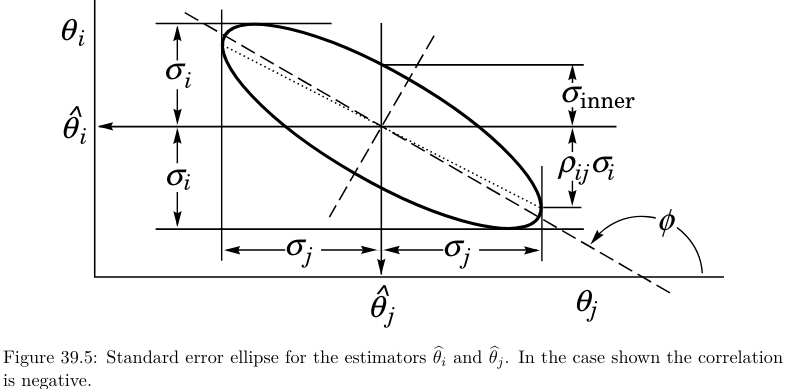
\includegraphics[width=0.9\textwidth,keepaspectratio]{estimatorvar}
	\label{fig:}
\end{figure}
contours in parameter space whose tangents are $\hat{\theta}_i\pm\hat{\sigma}_i$: $\chi^2(\vec{\theta})=\chi^2(\hat{\theta})+1$.
\end{frame}

\begin{frame}{Esempi di LS estimators}
\begin{itemize}
\item Combine many measures $y_i$ of $\lambda$ with estimated error $\sigma_i$: $\hat{\lambda}=\frac{\sum_iy_i/\sigma_i^2}{\sum_i1/\sigma_i^2}$, $\var[\hat{\lambda}]=\frac{1}{\sum\frac{1}{\sigma_i^2}}$; for not independent measures:
\begin{align*}
&\chi^2(\lambda)=\sum_{i,j}(y_i-\lambda)(\invers{V})_{i,j}(y_j-\lambda)\\
&w_i=\frac{\sum_j(\invers{V})_{ij}}{\sum_{k,l=1}\invers{V}_{kl}},\ \hat{\lambda}=\sum_iw_iy_i\\
&\var{[\hat{\lambda}]}=\sum_{i,j}w_iV_{ij}w_j
\end{align*}
\end{itemize}
\end{frame}

\subsection{Robustezza}

\begin{frame}{Outliers. Incertezza sistematica.}
I dati seguono una pdf a meno di $\epsilon$: $p_{tot}=(1-\epsilon)p_{th}+\epsilon q_{sys}()$
All'aumentare del numero di eventi di un rivelatore di particelle l'incertezza statistica diminuisce quindi diventa rilevante incertezza sistematica: si considerano stimatori del tipo $\min\sum|x_i-\hat{m}_p|^p$
\begin{block}{Costruzione stimatori robusti (distribution indipendent)}
Location-scale model observation $x_i=\mu+\sigma\epsilon_i$ (if $\epsilon_i$ iid Cauchy expected value doesn't exist)
Parametro di localizzazione e scala (sample mean and variance under normality assumption) invariante per:
\begin{align*}
&T_n(ax_1+b,\ldots,ax_n+b)=aT_n(x_1,\ldots,x_n)+b\\
&S_n(ax_1+b,\ldots,ax_n+b)=|a|S_n(x_1,\ldots,x_n)
\end{align*}
\end{block}
\end{frame}

\begin{frame}{Stimatori robusti}
\begin{itemize}
\item Mediana campionaria: $\min\sum|x_i-\hat{m}_1|$: $P(x<\hat{m}_1)=\prob{(x>\hat{m}_1)}$. MLE per $p(x,m)=\exp{-|x-m|}$. $T_n=\med{}$
\item Stimatore di mid-range: $\lim_{p\to\infty}\min\sum|x_i-\hat{m}_{\infty}|^p=\frac{x_M-x_m}{2}$
\item Moda:	$\lim_{p\to-\infty}\min\sum|x_i-\hat{m}_{-\infty}|^p$ seleziona coppia di dati pi\'u vicini.
\item Dispersion estimator (MAD): $c\med{}_i|x_i-\med{}_jx_j|$
\end{itemize}
\end{frame}

\begin{wordonframe}{Ex: Inferenza probabilistica}
\keyword{Ex: compito a risposta multipla} con  5 opzioni
\begin{itemize}
\item Studente a risponde a caso: $P_G=1/5$.
\item Studente B ipotizza distribuzione uniforme delle risposte attorno al valore giusto: sceglie la mediana. $P_B=5\frac{1}{5}\binom{4}{2}(\frac{1}{2})^2(1-\frac{1}{2}){4-2}=\frac{3}{8}$
\item \keyword{Ex: Studente usa MLE per pdf uniforme}
\end{itemize}

\end{wordonframe}

\begin{wordonframe}{Confronto fra stimatori per pdf contaminata}
Per gaussiana confronto $S_N=\frac{\sum(x_i-\exv{x})^2}{N}$, $d_N=\frac{\sum|x_i-\exv{x}|}{N}$ ($\lim_{N\to\infty}\E{[d_N]}=\sqrt{\frac{2}{\pi}}\sigma$): $r=\lim_{N\to\infty}\frac{\var{[S_N]}}{\var{[d_N']}}=0.876$.
\end{wordonframe}

\begin{wordonframe}{Distribuzione di probabilit\'a della mediana campionaria}
Per $2N+1$ misure la probabilit\'a che la misura $N+1$-esima misura sia $m_1$ \'e \[\prob{(m_1)}=\prob_x{(m_1)}F_x(m_1)^N(1-F_x(m_1)^N(2N+1)\binom{2N}{N}\] cio\'e la "densit\'a di probabilit\'a" che una misura cada in $m_1$ moltiplicata per $(2N+1)$ estrazioni, per la probabilit\'a che N misure stiano sotto e N sopra tenendo conto delle $\binom{2N}{N}=\frac{(2N)!}{(2N-N)!N!}$ ways to choose N elements between 2N (che coincide con disposizioni con ripetizioni). Per estrazioni con pdf di Cauchy:
\begin{align*}
&\prob{(\hat{m}_1)}=\frac{1}{1+m^2}[\frac{1}{4}-\frac{\arctan{(m_1)}^2}{\pi^2}]^N\\
&\var{\hat{m}_1}=\intsinf{}\frac{m^2}{m^{k+2}}\,dm
\end{align*}
Cambio di variabile: $y=F(\hat{m}_1)$, con $F(m_1)=\frac{1}{2}$ e $y\approx\frac{1}{2}+f(\hat{m}_1)(\hat{m}_1-m)$
\begin{align*}
&p(y)=\frac{(2n+1)!}{n!n!}y^n(1-y)^ndy,\ dy=f(m_1)dm_1\intd{usando le funzioni $\beta$ e $\Gamma$}
&\Gamma=\intzi{}t^{x-1}\exp{-t}\,dt,\ \beta(x,y)=\int_0^1t^{x-1}(1-t)^{y-1},\ \Gamma(x)\Gamma(y)=\Gamma(x+y)\beta(x,y)\\
&\prob{(y)}\propto\frac{x^{m-1}(1-y)^{n-1}}{\beta(m,n)}\\
&\E{[x]}\propto\int_0^1\frac{x^m(1-x)^{n-1}}{B(m,n)}\,dx=\frac{m}{m+n},\ \E{[x^2]}=\frac{\beta(m+2,n)}{\beta(n,m)}\\
&\var{[x]}=\frac{mn}{(n+m+1)(n+m)^2},\ \var{[y]}=\frac{1}{4(2m+1)}\\
&\var{[\hat{m}_1]}\approx\frac{1}{4(N+2)}\frac{1}{f^2(m_1)}
\end{align*}
\end{wordonframe}

\begin{wordonframe}{Come capire se la pdf \'e asintoticamente gaussiana?}
La distribuzione \'e asintoticamente gaussiana?? $\sqrt{N}(y-\E{[y]})\to N(0,\var{y})$.
\begin{columns}[T]
\begin{column}{0.5\textwidth}
\begin{align*}
&x_i\to z_i\to y=\frac{1}{N}\sum z_i\\
&z_i=\left\{\begin{matrix}1\ x<\hat{m}_1\\0\ x>\hat{m}_1\\\end{matrix}\right.\\
&\sqrt{N}(y-\var{(y)})\xrightarrow{\prob{}}N(0,\var{(y)})
\end{align*}
\end{column}
\begin{column}{0.5\textwidth}
z ha pdf binomiale w $\var{(y)}=\frac{np(1-p)}{n^2}\xrightarrow{p=1/2}\frac{1}{4n}$: utilizzando espansione di $y$ trovo espressione asintotica $\var{\hat{m}_1}=\frac{1}{4n^2}f^2(m_1)$, per $p\neq\frac{1}{2}$ $\var{(m_{\%})}=\frac{p(1-p)}{nf^2(\hat{m_{\%}})}$
\end{column}
\end{columns}

\keyword{Ex: Pdf di irwin-hall \'e asintoticamente gaussiana?}-Pdf uniforme centrata in $x_0$ e larga $\Delta$: trovare pdf di moda, mediana e midrange.

\keyword{Ex: Efficienza stimatori. Mediana vs MLE per pdf di Cauchy.}
pdf $f(x)=\frac{1}{\pi\gamma[1+(\frac{x-x_0}{\gamma})^2]}$:
\begin{columns}[T]
\begin{column}{0.5\textwidth}
Mediana
$\E{[\hat{m}_1]}=x_0, \var{(\hat{m}_1)}=\frac{\pi^2\gamma}{4n}$
\end{column}
\begin{column}{0.5\textwidth}
MLE:
\begin{align*}
&\sum^N\frac{\gamma^2}{\gamma^2+(x_i-x_0)^2}-\frac{h}{2}=0\\
&\var{(\hat{MLE})}=\frac{2}{N}\gamma^2:\ \epsilon=\frac{8}{\pi^2}\approx81\%
\end{align*}
\end{column}
\end{columns}

\keyword{Confronto Stimatori: $L_P(\alpha)=\sum^N|x_i-\alpha|^P$}
\begin{tabular}{c|ccc}
Unif & $\frac{1}{4N}$ & $\frac{1}{12N}$ & $\frac{1}{2(N^2+6N+4)}$\\
Triang & & $\frac{1}{6N}$ & $4-\frac{\pi}{4N}$\\
Norm & $\frac{\pi}{2N}$ & $\frac{1}{N}$ & $\frac{\pi^2}{12\ln{N}}$\\
DE & $\frac{1}{2N}$ & $\frac{2}{N}$ & $\frac{\pi^2}{12}$\\
Cauchy & $\frac{\pi^2}{4N}$ & & \\
\end{tabular}\end{wordonframe}

\begin{wordonframe}{Alcune propriet\'a dei parametri di localizzazione}
\begin{block}{Relazioni tra media, mediana e moda}
\begin{align*}
&|\mu-m_1|=|\E{[x-\hat{m}_1]}|\leq\E{[|x-\hat{m}|]}\leq\sqrt{\E{[(x-\hat{m})^2]}}=\sigma\\
&|m_1-m_{-\infty}|\leq\sqrt{3}\sigma
\end{align*}
\end{block}
\end{wordonframe}

\section{Stima intervallare}\linkdest{interval}

\begin{frame}{Short-coming of point-like estimators}
For suff. large samples  point estimate and standard deviation provide: objective comunication of results, interval containing on average the true param, 
Otherwise, (or non gaussian estimators, physical boundary for parameters) one have to use frequentist confidence interval and/or Bayesian credible interval.
\end{frame}

\subsection{Credibility intervall (bayesiano)}

\begin{frame}[fragile]{Bayesian credibility Interval}
\keyword{Intervallo di Credibilit\'a (Bayesiano)}: l'integrale della posterior sull'intervallo \'e $CL$, probabilit\'a che l'intervallo contenga il valore vero del parametro.
\begin{block}{\keyword{Ordinamento (Funzione di)}}
	determina la maniera in cui costruisco la regione di credibilit\'a: $+x$, $-x$, $\prob{x}$ possono essere funzioni di ordinamento - l'integrazione parte dal valore maggiore
\end{block}
\end{frame}

\begin{frame}{}
\begin{block}{\keyword{Credibility (della posterior)}}
	\begin{align*}
	&\cred{(x)}=\int_{\mu\in\inf(x)}\Pi(\mu|x)\,d\mu=\int_{\mu\inf(x)}\frac{\prob{(x|\mu)}\prob{(\mu)}}{\int\,d\mu}\,d\mu>\cl{}
	\end{align*}
\end{block}
	\begin{picture}(100,130)
	\put(20,20){
		\begin{tikzpicture}[scale=0.4]
		\def\basefunc{exp(-(x-1)^2)}
		\begin{axis}[title={central},name=central,samples=50,ymin=0,xmin=-2,xmax=4,xlabel={$m$},ylabel={$\prob{(m|x_0)}$}]
		\addplot gnuplot [no marks,domain={-2:0}]{\basefunc} \closedcycle; 
		\addplot gnuplot [no marks,domain={2:4}]{\basefunc} \closedcycle; 
		\addplot gnuplot [black,thick,fill=grey,smooth,no marks,domain={0:2}]{\basefunc} \closedcycle;
		\node (unomenocl) at (axis cs:-1,0.3) {$1-\frac{\alpha}{2}$};
		\end{axis}
		\hspace{0.5cm}
		\begin{axis}[title={upper limit}, at={($(central)+(4.5cm,-3cm)$)},name=upper,samples=50,ymin=0,xmin=-2,xmax=4,xlabel={$m$},ylabel={$\prob{(m|x_0)}$}]
		\addplot gnuplot [no marks,fill=grey,domain={-2:2}]{\basefunc} \closedcycle; 
		\addplot gnuplot [black,thick,smooth,no marks,domain={2:4}]{\basefunc};   
		\end{axis}
		\edef\oprob{0.47}
		\hspace{0.5cm}
		\begin{axis}[at={($(upper)+(4.5cm,-3cm)$)}, title={probability order},name=central,samples=50,ymin=0,xmin=-2,xmax=4,xlabel={$m$},ylabel={$\prob{(m|x_0)}$}]
		\addplot[name path=prob] gnuplot[grey,thick,smooth,no marks]{\oprob};
		\addplot[name path=gauss] gnuplot[black,thick,smooth,no marks]{\basefunc};
		\path [name intersections={of=gauss and prob ,by={Pa,Pb}}];
		\node[above left] at (Pa) {$x_-$} node[above right] at (Pb) {$x_+$};
		\pgfkeys{/pgf/fpu=true}
		\pgfmathparse{1-sqrt(-ln(\oprob))}
		\def\xleft{\pgfmathresult}
		\pgfmathparse{1+sqrt(-ln(\oprob))}
		\def\xright{\pgfmathresult}
		\pgfmathparse{1+sqrt(-ln(\oprob))}
		\pgfkeys{/pgf/fpu=false}
		\addplot gnuplot [no marks,fill=grey,domain={0.13:1.87}]{\basefunc} \closedcycle; 
		\node (unomenocl) at (axis cs:0,0.7) {$CL$};
		\end{axis}
		\end{tikzpicture}}
	\end{picture}
\end{frame}

\subsection{Confidence interval (frequentista)}

\begin{frame}{\keyword{Neyman construction}. Frequentist confidence intervals}
\keyword{Confidence interval (frequentista)}: molte ripetizioni dell'esperimento, CL volte l'intervallo contiene il parametro.
%reminder: banda confidenza con pgfplot/gnuplot
\begin{columns}[T]
\begin{column}{0.4\textwidth}
	\begin{figure}
		\centering
		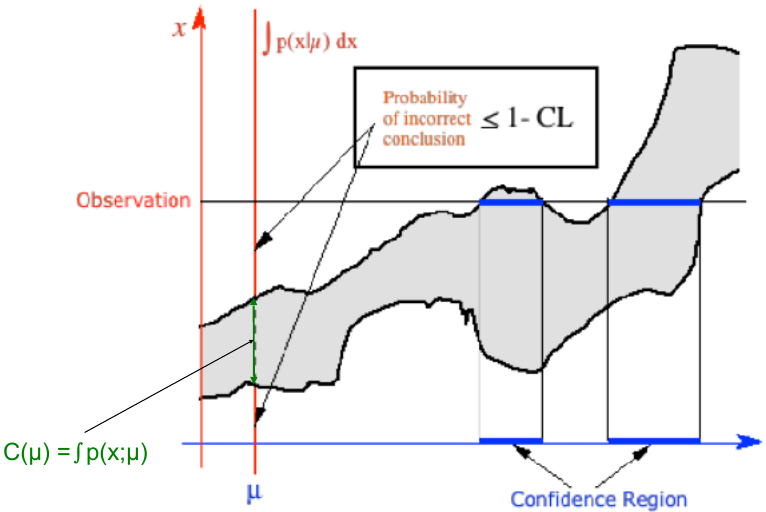
\includegraphics[width=0.9\textwidth,keepaspectratio]{clband}
		\label{fig:clband}
	\end{figure}
	\begin{figure}
		\centering
		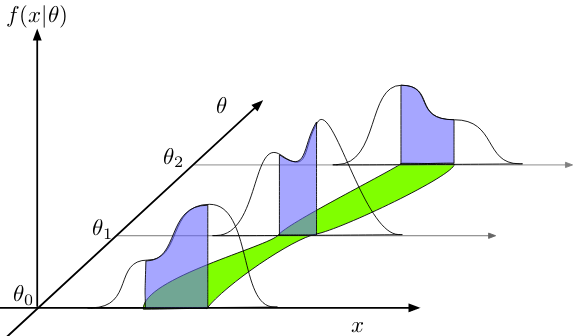
\includegraphics[width=0.9\textwidth,keepaspectratio]{neyman}
		\label{fig:neyman}
	\end{figure}
\end{column}
\begin{column}{0.6\textwidth}
	\begin{block}{Costruzione di Neyman}
		\keyword{Coverage}: $\coverage{(\mu)}=\int_{x:\mu\in f(x)}\prob{(x;\mu)}\,dx$, $f(x)$ associa un intervallo nello spazio dei parametri a una misura; l'algoritmo ha livello di confidenza $\cl=\inf_{\mu\in A}C(\mu)$ cio\'e l'intervallo associato alla data misura ha probabilit\'a $\cl{}$ di contenere il parametro: con misure ripetute $\cl$ volte l'intervallo contiene il parametro.
	\end{block}
	\begin{block}{Ordering}
		''The way I integrate over the data''
	\end{block}
\end{column}
\end{columns}
\end{frame}

\begin{wordonframe}{Workout funzione di coverage}
\keyword{Coverage in frequentist approach}: \'e propriet\'a del metodo not of any particular interval.
Graphical Methods for Evaluating and ComparingConfidence-Interval Procedures
\end{wordonframe}

\begin{frame}{Feldman-Cousins unified approach}\frameintoc
\begin{columns}[T]
\begin{column}{0.5\textwidth}
%insactisfaction with Neyman construction for upper limit in case of empty/unphysical interval
\keyword{Shortcoming of Neyman}: flip-flop problem, ie using upper limit and central limits after seeing the data may not cover; empty interval: the method has exact coverage even if empty interval don't cover true param
\keyword{Feldman-Cousins unified approach}: LR-ordering $R=\frac{\prob{(x;\mu)}}{\prob{(x;\mu_{best})}}$, values of x/n are added to acceptance region as decreasing function of R.
Confidence interval: $R(m_1)=R(m_2)$
\end{column}
\begin{column}{0.5\textwidth}
\begin{figure}[!ht]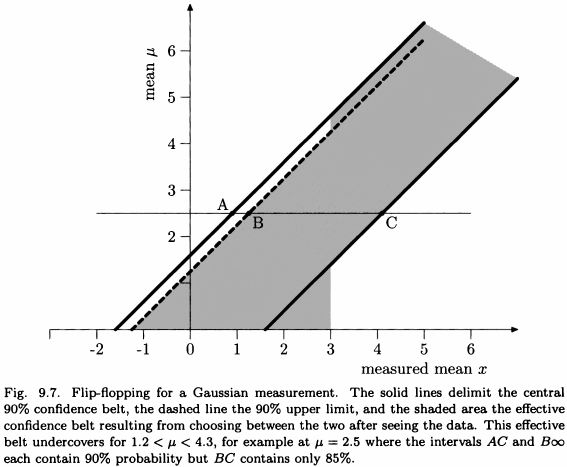
\includegraphics[trim={0cm 0cm 0 0},clip, keepaspectratio,height=0.49\textheight]{flipflopping}\label{fig:pdfestexp}\end{figure}
\end{column}
\end{columns}

\end{frame}

\begin{frame}{Stima intervallare bayesiana/frequentista per $U([0,m])$ (una misura)}

\begin{columns}[T]
\begin{column}{0.5\textwidth}
\def\myscale{0.4}
\begin{tikzpicture}[myscalar]
\begin{axis}[title={Banda di credenza per $U([0,m])$},name=uniformcredence,ymin=0,xmin=0,xmax=6,xlabel={$m$},ylabel={$x$},y label style={rotate=-90, at={(-0.1,1.)}},extra x tick style={% changes for extra x ticks
tick label style={yshift=-4mm}},
%extra x tick labels={$x\exp{1-\alpha}$},extra x tick labels={$x\exp{1-\alpha}$},
extra y ticks={0.5},extra y tick labels={measure $x_0$}]
\addplot[name path global=om, no marks] gnuplot[id=upperbound,domain=0:6] {x};
\addplot[name path global=op, no marks] gnuplot[id=lowerbound,domain=0:6] {x*exp(-1+0.05)};
\addplot[name path global=meas,dash pattern=on 4pt off 3pt,no marks,samples=10,black,thin] gnuplot[domain=0:6] {0.5};
\end{axis}
\end{tikzpicture}
\def\myscale{0.4}
\begin{tikzpicture}[myscalar]
\begin{axis}[title={Banda confidenza $U([0,m])$},name=uniformconfidence,ymin=0,xmin=0,xmax=8,xlabel={$m$},ylabel={$x$},y label style={rotate=-90, at={(-0.1,1.)}},extra x tick style={% changes for extra x ticks
tick label style={yshift=0mm}},extra y ticks={0.3},extra y tick labels={measure $x_0$}]
\addplot[name path global=bp, no marks] gnuplot[id=upperbound,domain=0:8] {x*(1-0.9)};
\addplot[name path global=bm, no marks] gnuplot[id=lowerbound,domain=0:8] {x};
\addplot[name path global=meas,dash pattern=on 4pt off 3pt,no marks,black] gnuplot[domain=0:8] {0.3};
\path[name intersections={of={bp and meas},name=i},name intersections={of={bm and meas},name=j}] (i-1) (j-1);
\pgfplotsextra{\path (i-1) \pgfextra{\markxof{i-1}\xdef\myfirsttick{\pgfmathresult}}(j-1); \pgfextra{\markxof{j-1}\xdef\mysecondtick{\pgfmathresult}};
}
\end{axis}
\draw[ultra thin, draw=gray] (i-1 |- {rel axis cs:0,0}) node[fill=yellow,yshift=-1ex]{\pgfmathprintnumber[fixed,precision=5]\myfirsttick} -- (i-1);
\draw[ultra thin, draw=gray] (j-1 |- {rel axis cs:0,0}) node[fill=red,below]{\pgfmathprintnumber[fixed,precision=5]\mysecondtick} -- (j-1);
\end{tikzpicture}
\end{column}
\begin{column}{0.5\textwidth}
La banda di confidenza si costruisce integrando sulla distribuzione dell'osservabile su una regione tale che l'integrle sia il livello di confidenza $\cl=1-\alpha$.

L'intervallo di credibilit\'a \'e definito dalla banda per cui ''l'integrale della likelihood per dato valore dell'osservabile'' \'e $1-\alpha$.

\end{column}
\end{columns}
\end{frame}

\begin{wordonframe}{Stima intervallare bayesiana/frequentista per $U([0,m])$: statistica sufficiente}
\begin{block}{Statistica sufficiente $x_M$}
\keyword{workout: pensare a relazione tra misura osservabile, bande di confidenza e statistiche sufficienti}: Nel caso uniforme ho una sola statistica sufficiente $x_{max}$ - posso ridurre la banda di confidenza per N misure a intervallo di confidenza utilizzando $x_{max}$.
\end{block}

La distribuzione di probabilit\'a della statistica sufficiente $x_M$ \'e $\prob{(x;m)}=\frac{N}{m}(\frac{x}{m})^{N-1}$:
\begin{columns}[T]
\begin{column}{0.5\textwidth}
''L'algoritmo di ordinamento'' su valori osservabile determina la forma dell'intervallo di confidenza
\end{column}
\begin{column}{0.5\textwidth}
Ordinamento:
$+x$ - upper limit - $m<\frac{x_M}{1-\cl}$, $-x$ - lower limit $m>\cl{}x_M$, probability ordering - no, central interval $m\in[\frac{2x_M}{1+\cl{}},\frac{2x_M}{1-\cl{}}]$
\end{column}
\end{columns}
\end{wordonframe}

\begin{wordonframe}{Ordinamento su LR per bande confidenza pdf uniforme}
LR: upper limit - $m<\frac{x_M}{1-\cl{}}$
\begin{columns}[T]
\begin{column}{0.5\textwidth}
\begin{align*}
&\lr{}=\frac{\prob{(x_M;m)}}{\sup_m{\prob{(x_M;m)}}}\\
&=\frac{\frac{N}{m}(\frac{x}{m})^{N-1}}{N/m}=(\frac{x}{m})^N
\end{align*}
\keyword{Funzione $\lambda$}: $\lambda=-2\log{\lr{}}=-2N\log{\frac{x}{m}}$
\end{column}
\begin{column}{0.5\textwidth}
likelihood decresce sempre con m (dove $\PDy{m}{L}=0$?). \keyword{Inconsistenza nella definizione di bande di confidenza con $o=\lr{}$?} (Likelihood funzione di m).
La banda \'e identificata da $\lr\geq q_{\cl{}}$
\end{column}
\end{columns}
Determino $\prob{(\lambda)}$: cambiamento variabile $\left\{\begin{array}{c}
u=\frac{x}{m}\\
v=\log{u}\\
\lambda=-2Nv\\
\end{array}\right.$
\begin{align*}
&\prob{(u;m)}=\frac{\prob{(x(u);m)}}{|\TDy{x}{u}|_{x(u)}}=Nu^{N-1}\\
&\prob{(v;m)}=\frac{\prob_u{(u(v);m)}}{|\TDy{u}{v}|_{u(v)}}=N\exp{Nv}\\
&\prob{(\lambda;m)}=\frac{1}{2}\exp{-\frac{\lambda}{2}}
\end{align*}
Integrale di coverage:
\begin{align*}
&\cl=\int_{\lr>q_{\cl}}\prob{(x_M;m)}\,dx_M=\int_{\lambda<q_{\cl}'}\prob{(\lambda;m)}\,d\lambda\\
&\Rightarrow \left\{\begin{array}{c}
m\in[1,\frac{1}{\sqrt[N]{1-\cl}}]x_M (F)\\
N>1:\ m\in[1,\frac{1}{\sqrt[N-1]{1-\cl}}]x_M (B)\\
\end{array}
\right.
\end{align*}
\keyword{Ex: Credibility LR-ordering $U$}
\end{wordonframe}

%% banda di confidenza per distribuzione uniforme

\subsection{Pivotal quantities}\linkdest{pivot}

\begin{frame}{Pivot}
Pivot: RV $U(T,\theta)$ funzione di statistica sufficiente e parametro ma la distribuzione di U non dipende dal parametro $\forall \theta\in\Theta$ (asymptotic if true for $n\to\infty$).
\begin{align*}
&p(x;\mu)=\frac{1}{\sqrt{2\pi}\sigma}\exp{-\frac{(x-\mu)^2}{2\sigma^2}}\\
&(s=\frac{x-\mu}{\sigma}:\ p(s;\mu)=N(0,1)\\
&\int_{s>c}p(s)\,ds=\cl{}=1-\alpha
\end{align*}
\keyword{Pivot. 2-sided CI for exponential}:
\begin{align*}
&f(x;\theta)=\invers{\theta}\exp{-\frac{x}{\theta}}I(x>0)\ \to\ g(u)=\exp{-u}I(u>0)\\
&\prob{(a<u<b)}=1-\alpha\Rightarrow\prob{(\theta\in(\invers{b}x,\invers{a}x))}=1-\alpha\ (\alpha\leftrightarrow1-\alpha)
%
\end{align*}
\end{frame}

\begin{wordonframe}{Example of CI using Pivot}

\end{wordonframe}

\begin{wordonframe}{Esempi intervalli di confidenza e credibilit\'a}
\begin{block}{Limite superiore Poisson con $k=0$}
$\prob{(k|\mu)}=\frac{\mu^k\exp{-\mu}}{k!}$: registro $k=0$ conteggi, ricavo limite superiore frequentista e bayesiano per $\mu$
\end{block}
\keyword{Ex: limite superiore bayesiano per Poisson} - La posterior $\prob{(\mu|0)}=\exp{-\mu}$ per $\cl{}=\alpha\%$ si ha $\int_0^{\mu_u}\exp{-\mu}\,d\mu=\alpha$, per $\cl{}=90\%$ si ha $\mu<2.3@90\%\cl{}$.
\begin{columns}[T]
\begin{column}{0.5\textwidth}
\keyword{Ex: limite superiore frequentista per Poisson} - Upper limit: $\sum_{k_{min}}^{\infty}\prob{(k|\mu)}=\alpha$; $\prob{(0|\mu)}=0.1 (=1-\alpha)$ per $\mu_0=\ln{10}$, $\prob{(0|\mu_1)}+\prob{(1|\mu_1)}=0.1$ per $\mu_1=3.89$, $\prob{(0|\mu_1)}+\prob{(1|\mu_1)}+\prob{(2|\mu_1)}=0.1$ per $\mu_2=5.32$
\end{column}
\begin{column}{0.5\textwidth}
\begin{picture}(100,130)
\put(20,20){
\begin{tikzpicture}[scale=0.4]
\begin{axis}[title={Coverage},name=central,samples=50,ymin=0,xmin=0,xmax=6,xlabel={$\mu$},ylabel={$k$},y label style={rotate=-90, at={(-0.1,1.)}},extra x ticks={2.3,3.89,5.32},extra x tick style={% changes for extra x ticks
tick label style={yshift=-4mm}},
extra x tick labels={$\mu_0$, $\mu_1$, $\mu_2$},extra y ticks={0},extra y tick labels={measure $k=0$}]
\addplot+[name path=dwcover,const plot, no marks, thick] coordinates {(0,0) (2.3,1) (3.89,2) (5.32,3)};
\addplot[quiver={u=0,v=x>2.3 ? (x>3.9 ? -1 : -2):-3},-stealth, samples=15] {3}; 
\end{axis}
\end{tikzpicture}}
\end{picture}	
\end{column}
\end{columns}
\keyword{Ex: Poisson con $k=0,1,2$ conteggi e ordinamento LR, Up, Down, Central} 
\keyword{Ex: Limiti bayesiani e frequentisti sul numero di facce dadi D\&D estrazioni 1,1} - $S=\{4,6,8,10,12,20\}$:
\begin{columns}[T]
\begin{column}{0.5\textwidth}
\keyword{T bayes (lancio 6 dadi)} $\pgfkeys{/pgf/fpu=true}\prob{(1)}=\sum_i\prob{(D_i)}\prob{(1|D_i)}=\xdef\Sum{0}
\foreach \i in {4,6,8,10,12,20} {\xdef\Sum{\Sum+1/(6*\i)}}\pgfmathparse{\Sum}\pgfmathprintnumber{\pgfmathresult}\pgfkeys{/pgf/fpu=false}$
Limite superiore al numero di facce: $\sum_{\mu}\prob{(x_0;\mu)}\geq1-\alpha$, $n_f\leq12$ at $\cl>90\%$
\end{column}
\begin{column}{0.5\textwidth}
\pgfkeys{/pgf/fpu=true}
\pgfmathparse{(1/4)*(1/6)*(1/0.1292)}\pgfmathsetmacro{\postfour}{\pgfmathresult}
\pgfmathparse{(1/6)*(1/6)*(1/0.1292)}\pgfmathsetmacro{\postsix}{\pgfmathresult}
\pgfmathparse{(1/8)*(1/6)*(1/0.1292)}\pgfmathsetmacro{\posteight}{\pgfmathresult}
\pgfmathparse{(1/10)*(1/6)*(1/0.1292)}\pgfmathsetmacro{\postten}{\pgfmathresult}
\pgfmathparse{(1/12)*(1/6)*(1/0.1292)}\pgfmathsetmacro{\posttwelve}{\pgfmathresult}
\pgfmathparse{(1/20)*(1/6)*(1/0.1292)}\pgfmathsetmacro{\posttwenty}{\pgfmathresult}
\pgfkeys{/pgf/fpu=false}
\begin{tikzpicture}[scale=0.5]
\begin{axis}[
ybar stacked,
bar width=15pt,
nodes near coords% = {%
%\pgfmathprintnumberto[fixed,assume math mode=true]{\pgfplotspointmeta}{\myval}%
%\pgfmathparse{\myval<0.05?:\myval}\pgfmathresult%}
,
enlargelimits=0.2,
ylabel={$\prob{(D_i|1)}$},
symbolic x coords={d4, d6, d8, d10, d12, d20},
xtick=data,
x tick label style={anchor=north},
xticklabels={$D_4$, $D_6$, $D_8$, $D_{10}$, $D_{12}$, $D_{20}$},cycle list name = ColorListBar
]
\addplot+[ybar] plot coordinates {(d4,\postfour) (d6,\postsix) (d8,\posteight) (d10,\postten) (d12,\posttwelve) (d20,\posttwenty)};
\end{axis}
\end{tikzpicture}
Probability ordering (Cosa vuol dire ordinamento?)
\end{column}
\end{columns}
\begin{columns}[T]
\begin{column}{0.3\textwidth}
\begin{tikzpicture}[scale=0.3]
\begin{axis}[
ybar stacked,
bar width=15pt,
nodes near coords% = {%
%\pgfmathprintnumberto[fixed,assume math mode=true]{\pgfplotspointmeta}{\myval}%
%\pgfmathparse{\myval<0.05?:\myval}\pgfmathresult%}
,
enlargelimits=0.2,
ylabel={$\prob{(D_i)}$},
symbolic x coords={d4, d6, d8, d10, d12, d20},
point meta=explicit symbolic,
xtick=data,
ytick={4,6,8,10,12,20},
x tick label style={anchor=north},
xticklabels={$D_4$, $D_6$, $D_8$, $D_{10}$, $D_{12}$, $D_{20}$},cycle list name = ColorListBar,every node near coord/.append style={font=\tiny}
]
\addplot+[ybar] plot coordinates {(d4,4)[$1/4$] (d6,4) [$4/6$]
(d8,4)[$4/8$] (d10,4)[$4/10$] (d12,4)[$4/12$] (d20,4)[$4/20$]};
\addplot+[ybar] plot coordinates {(d4,16)[$0$] (d6,2) [$1$]
(d8,2)[$6/8$] (d10,2)[$6/10$] (d12,2)[$6/12$] (d20,2)[$6/20$]};
\addplot+[ybar] plot coordinates {(d4,0)[$0$] (d6,14) [$0$]
(d8,2)[$1$] (d10,2)[$8/10$] (d12,2)[$8/12$] (d20,2)[$8/20$]};
\addplot+[ybar] plot coordinates {(d4,0)[$0$] (d6,0) [$0$]
(d8,12)[$0$] (d10,2)[$1$] (d12,2)[$12/10$] (d20,2)[$20/10$]};
\addplot+[ybar] plot coordinates {(d4,0)[$0$] (d6,0) [$0$]
(d8,0)[$0$] (d10,10)[$0$] (d12,2)[$1$] (d20,2)[$20/12$]};
\addplot+[ybar] plot coordinates {(d4,0)[$0$] (d6,0) [$0$]
(d8,0)[$0$] (d10,0)[$0$] (d12,8)[$0$] (d20,8)[$1$]};
\end{axis}
\end{tikzpicture}
\end{column}
\begin{column}{0.7\textwidth}
limiti di confidenza frequentisti: costruzione banda di confidenza prendendo ordinamento sulla pdf di X a parametro dato. Limite superiore ordinando da 20 per estrazione 1 si ha $n_f\leq8$ con $\cl{}\geq90\%$
\end{column}
\end{columns}
\keyword{Ex: Dadi D\&D CI frequentista con LR ordering}
\end{wordonframe}

\subsection{Examples of estimator - exponential decay: MLE, distribution of estimator, change of variable, confidence interval}
%cowan 10.4

\begin{frame}{pdf per $\hat{\xi}$ da n misure indipendenti da distribuzione esponenziale}
\begin{columns}[T]\begin{column}{0.4\textwidth}
n misure indipendenti
\begin{align*}
&f(x;\xi)=\frac{1}{\xi}\exp{-\frac{x}{\xi}}\\
&\hat{\xi}_{MLE}=\frac{1}{n}\sum^nx_i
\end{align*}
\end{column}\begin{column}{0.6\textwidth}
If experiment repeated many times one would obtain $\hat{\xi}$ distributed as $g(\hat{\xi};n,\xi)$
\begin{align*}
&z=\sum^nx_i=n\hat{\xi}:\ \phi_x(t)=\frac{1}{(1-it\xi)^n}
\end{align*}
\end{column}\end{columns}
\begin{align*}
&g(\hat{\xi};n,\xi)=g_z(z)|\TDy{\hat{\xi}}{z}|=ng_z(n\hat{\xi})=\frac{n^n}{(n-1)!}\frac{\hat{\xi}\expy{n-1}}{\xi^n}\exp{-n\hat{\xi}/\xi}
\end{align*}
Special case of $\Gamma$ distribution
\begin{figure}[!ht]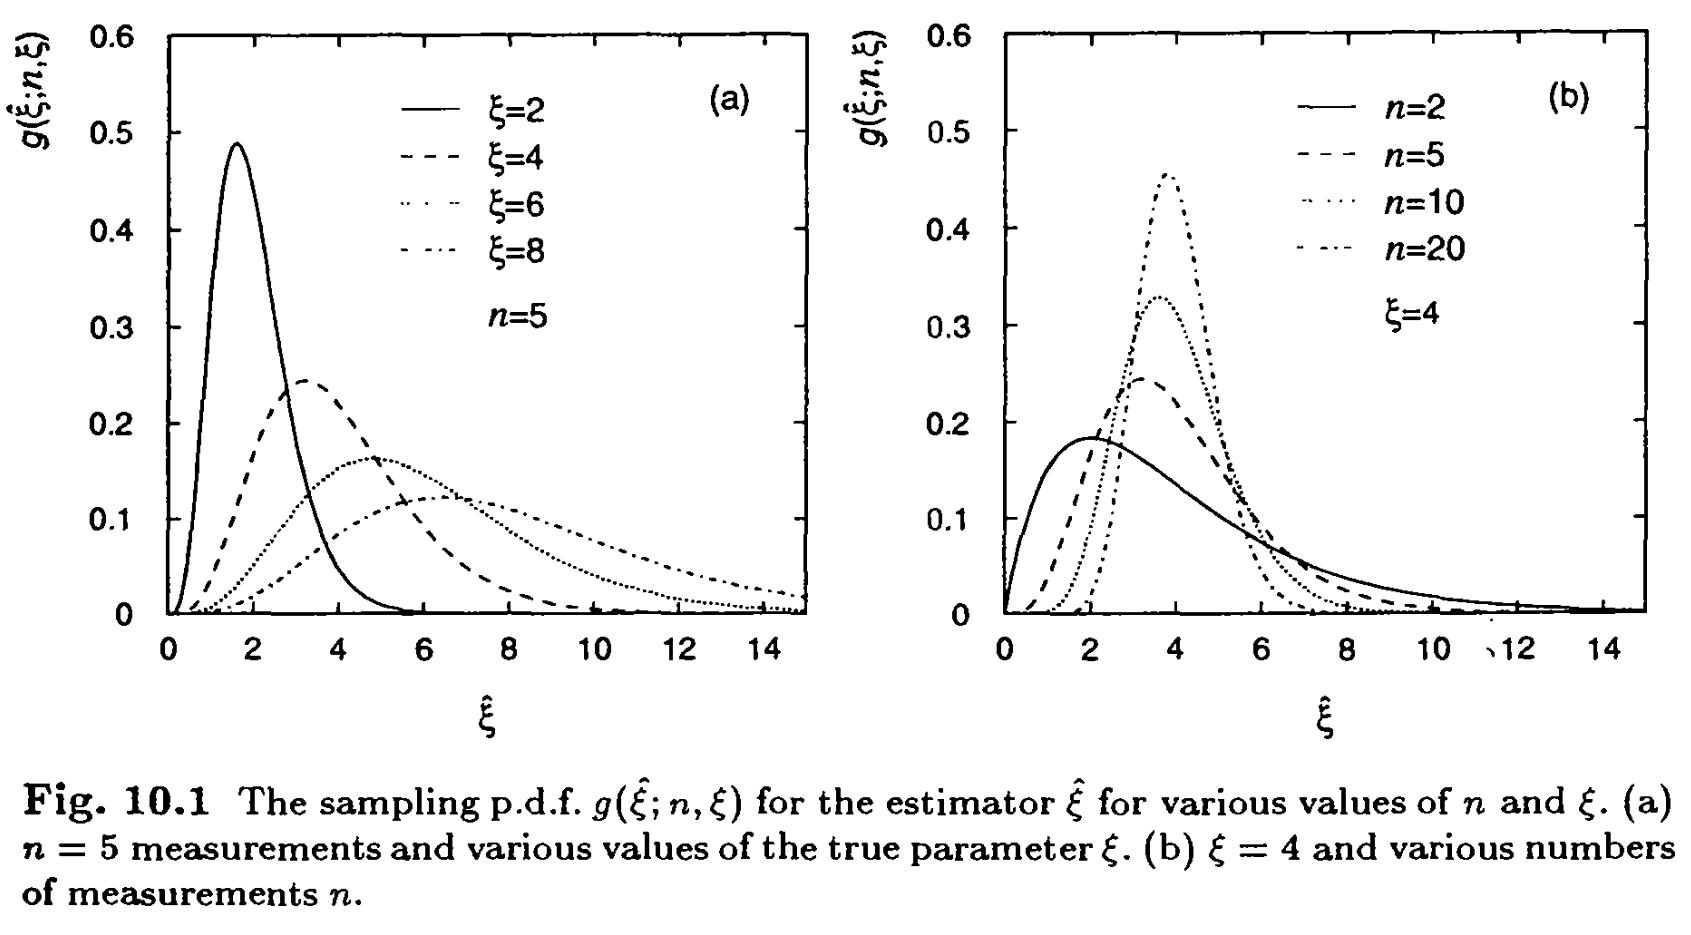
\includegraphics[trim={0cm 0cm 0 0},clip, keepaspectratio,height=0.4\textheight]{pdfestexp}\label{fig:pdfestexp}\end{figure}
\end{frame}

\begin{wordonframe}{Funzione caratteristica pdf esponenziale: Ripasso cambio di variabili e integrali nel piano complesso}
\begin{align*}
&\phi_x(t)=\int\exp{itx}f(x)\,dx\\
&(\oint_{\gamma}f(z)\,dz=2\pi i\sum I(\gamma,a_k)Res(f,a_k))\\
&\intzi{}\exp{itx}\frac{1}{\xi}\exp{-\frac{x}{\xi}}\,dx=\frac{1}{1-it\xi}\\
&z=\sum^nx_i=n\hat{\xi}:\ \phi_x(t)=\frac{1}{(1-it\xi)^n}\\
&g_z(z)=\frac{1}{2\pi}\intsinf{}\frac{\exp{-itx}}{(1-it\xi)^n}\,dt\xrightarrow{-i/\xi \text{ n-pole}}\frac{1}{(n-1)!}\frac{z\expy{n-1}}{\xi^n}\exp{-\frac{x}{\xi}}\\
\end{align*}
\end{wordonframe}

\begin{frame}{Expectation value for mean lifetime and decay constant}
\begin{block}{Tempo di decadimento}
$\hat{\tau}=\frac{1}{n}\sum^nt_i$: ritrovo il valore di aspettazione
\begin{align*}
&\E{[\hat{\tau}]}=\intzi{}\ldots\intzi{}(\frac{1}{n}\sum^nt_i)\frac{1}{\tau}\exp{-\frac{t_1}{\tau}}\ldots\frac{1}{\tau}\exp{-\frac{t_n}{\tau}}\,dt_1\ldots\,dt_n\\
&\E{[\hat{\tau}]}=\intzi{}\hat{\tau}g(\hat{\tau};n,\tau)\,d\hat{\tau}=\intzi{}\hat{\tau}\frac{n^n}{(n-1)!}\frac{\hat{\tau}\expy{n-1}}{\tau^n}\exp{-\frac{n\hat{\tau}}{\tau}}\,d\\hat{\tau}
\end{align*}
\end{block}
\begin{block}{Costante di decadimento}
\keyword{MLE for function of parameter} is same function of MLE of parameter:
\begin{align*}
&\hat{\lambda}=\frac{1}{\hat{\tau}}\\
&h(\hat{\lambda};n,\lambda)=g(\hat{\tau};n,\tau)|\TDy{\hat{\lambda}}{\hat{\tau}}|=\frac{n^n}{(n-1)!}\frac{\lambda^n}{\hat{\lambda}\expy{n+1}}\exp{-n\lambda/\hat{\lambda}}\\
&\E{[\hat{\lambda}]}=\intzi{}h(\hat{\lambda};n,\lambda)\hat{\lambda}\,d\hat{\lambda}=\frac{n}{n-1}\lambda
\end{align*}
\end{block}
\end{frame}

\begin{frame}{Confidence interval for mean of exponential RV}
n osservaqzioni di x per determinare lo stimatore $\hat{\xi}=\hat{\xi}_{obs}$ con pdf $g(\hat{\tau};n,\tau)=\frac{n^n}{(n-1)!}\frac{\hat{\xi}\expy{n-1}}{\xi^n}\exp{-n\hat{\xi}/\xi}$. Per determinare l'intervallo $[a,b]$ dati $x_1,\ldots,x_n$ devo risolvere
\begin{columns}[T]\begin{column}{0.4\textwidth}
\begin{align*}
&\alpha=\int_{\hat{\xi}_{obs}}^{+\infty}g(\hat{\xi};a)\,d\hat{\xi}\\
&\beta=\int_{-\infty}^{\hat{\xi}_{obs}}g(\hat{\xi};b)\,d\hat{\xi}
\end{align*}
\end{column}
\begin{column}{0.6\textwidth}
perfissati $\alpha,\beta$, indipendentemente dal vero $\xi$. Per $n\to\infty$ $g$ becomes gaussian (CLT) and $68.3\%$ central confidence interval approaches $[\hat{\xi}_{obs}-\hat{\sigma}_{\hat{\xi}},\hat{\xi}_{obs}+\hat{\sigma}_{\hat{\xi}}]$.
\end{column}
\end{columns}
\begin{figure}[!ht]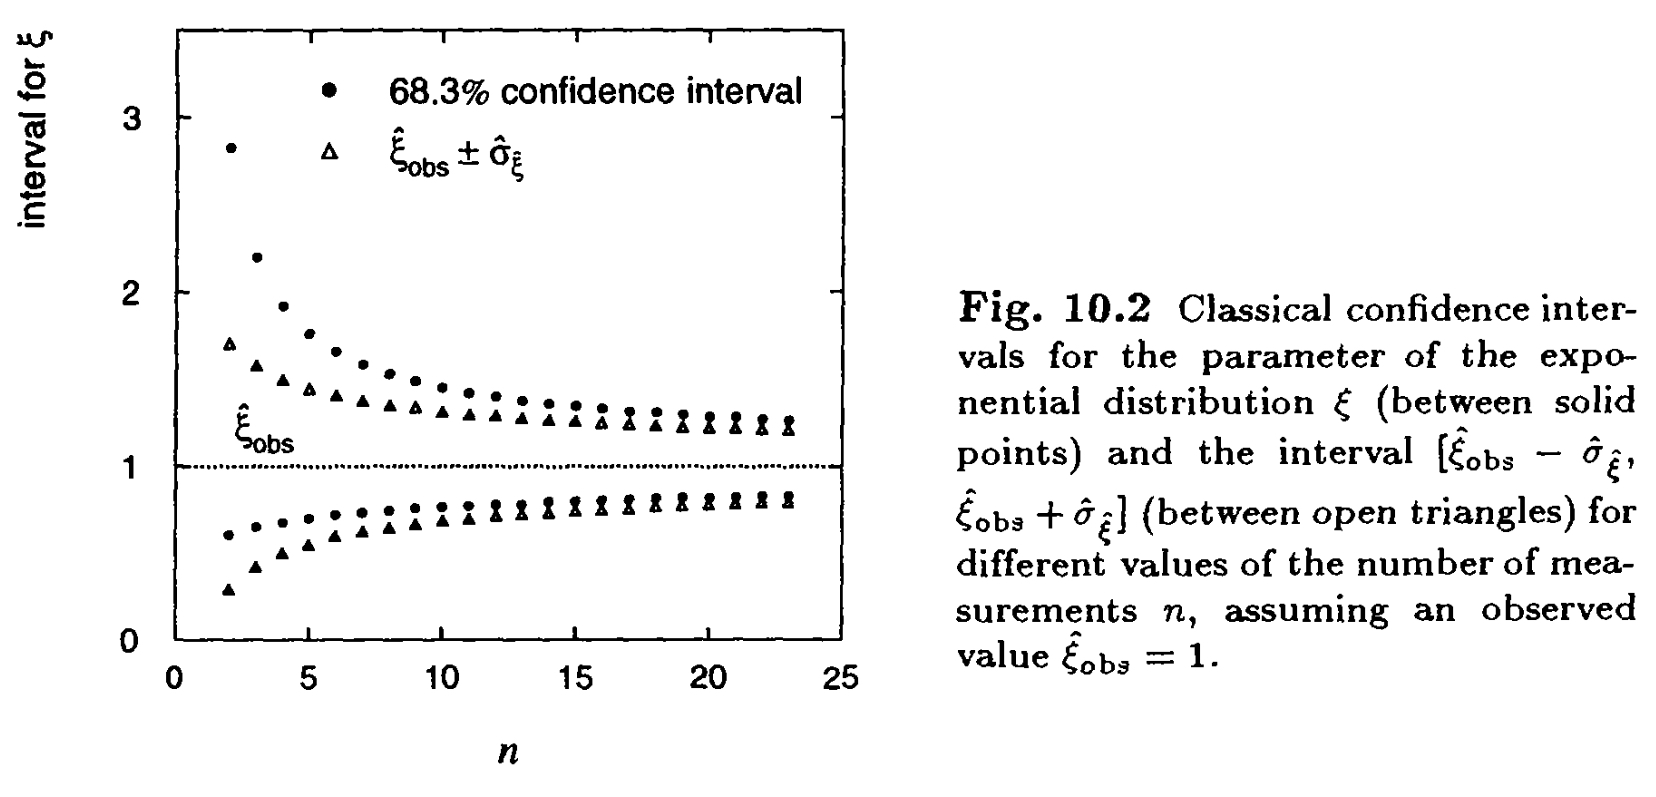
\includegraphics[trim={0cm 0cm 0 0},clip, keepaspectratio,height=0.4\textheight]{intestclt}\label{fig:intestclt}\end{figure}
\end{frame}

\subsection{Wilk's theorem}

\begin{frame}{Teorema di Wilks}\linkdest{wilks}\frameintoc
	$p(x;\mu)$ due volte differenziabile con dominio indipendente da parametro $\Omega(x;\mu)=\Omega(x)$: \[\lambda(x;\mu)=2\log{[\frac{\sup_{\mu}{p(x;\mu)}}{p(x;\mu)}]}\] (log-likelihood ratio statistics) ha asintoticamente pdf universale e indipendente da $\mu$: distribuzione di $\chi^2$ con dof pari a dimensione di $\vec{\mu}$.
	\begin{align*}
	&\ln{L(\theta)}-\ln{L(\hat{\theta})}=-\frac{1}{2}\invers{F}_{\chi_n^2}(1-\alpha)
	\end{align*}
\end{frame}